\documentclass[]{book}
\usepackage{lmodern}
\usepackage{amssymb,amsmath}
\usepackage{ifxetex,ifluatex}
\usepackage{fixltx2e} % provides \textsubscript
\ifnum 0\ifxetex 1\fi\ifluatex 1\fi=0 % if pdftex
  \usepackage[T1]{fontenc}
  \usepackage[utf8]{inputenc}
\else % if luatex or xelatex
  \ifxetex
    \usepackage{mathspec}
  \else
    \usepackage{fontspec}
  \fi
  \defaultfontfeatures{Ligatures=TeX,Scale=MatchLowercase}
\fi
% use upquote if available, for straight quotes in verbatim environments
\IfFileExists{upquote.sty}{\usepackage{upquote}}{}
% use microtype if available
\IfFileExists{microtype.sty}{%
\usepackage{microtype}
\UseMicrotypeSet[protrusion]{basicmath} % disable protrusion for tt fonts
}{}
\usepackage[margin=1in]{geometry}
\usepackage{hyperref}
\hypersetup{unicode=true,
            pdftitle={Introducción a los Diseños Experimentales con R},
            pdfauthor={Ana Vargas   e-mail:anavargas@lamolina.edu.pe},
            pdfborder={0 0 0},
            breaklinks=true}
\urlstyle{same}  % don't use monospace font for urls
\usepackage{natbib}
\bibliographystyle{apalike}
\usepackage{color}
\usepackage{fancyvrb}
\newcommand{\VerbBar}{|}
\newcommand{\VERB}{\Verb[commandchars=\\\{\}]}
\DefineVerbatimEnvironment{Highlighting}{Verbatim}{commandchars=\\\{\}}
% Add ',fontsize=\small' for more characters per line
\usepackage{framed}
\definecolor{shadecolor}{RGB}{248,248,248}
\newenvironment{Shaded}{\begin{snugshade}}{\end{snugshade}}
\newcommand{\KeywordTok}[1]{\textcolor[rgb]{0.13,0.29,0.53}{\textbf{#1}}}
\newcommand{\DataTypeTok}[1]{\textcolor[rgb]{0.13,0.29,0.53}{#1}}
\newcommand{\DecValTok}[1]{\textcolor[rgb]{0.00,0.00,0.81}{#1}}
\newcommand{\BaseNTok}[1]{\textcolor[rgb]{0.00,0.00,0.81}{#1}}
\newcommand{\FloatTok}[1]{\textcolor[rgb]{0.00,0.00,0.81}{#1}}
\newcommand{\ConstantTok}[1]{\textcolor[rgb]{0.00,0.00,0.00}{#1}}
\newcommand{\CharTok}[1]{\textcolor[rgb]{0.31,0.60,0.02}{#1}}
\newcommand{\SpecialCharTok}[1]{\textcolor[rgb]{0.00,0.00,0.00}{#1}}
\newcommand{\StringTok}[1]{\textcolor[rgb]{0.31,0.60,0.02}{#1}}
\newcommand{\VerbatimStringTok}[1]{\textcolor[rgb]{0.31,0.60,0.02}{#1}}
\newcommand{\SpecialStringTok}[1]{\textcolor[rgb]{0.31,0.60,0.02}{#1}}
\newcommand{\ImportTok}[1]{#1}
\newcommand{\CommentTok}[1]{\textcolor[rgb]{0.56,0.35,0.01}{\textit{#1}}}
\newcommand{\DocumentationTok}[1]{\textcolor[rgb]{0.56,0.35,0.01}{\textbf{\textit{#1}}}}
\newcommand{\AnnotationTok}[1]{\textcolor[rgb]{0.56,0.35,0.01}{\textbf{\textit{#1}}}}
\newcommand{\CommentVarTok}[1]{\textcolor[rgb]{0.56,0.35,0.01}{\textbf{\textit{#1}}}}
\newcommand{\OtherTok}[1]{\textcolor[rgb]{0.56,0.35,0.01}{#1}}
\newcommand{\FunctionTok}[1]{\textcolor[rgb]{0.00,0.00,0.00}{#1}}
\newcommand{\VariableTok}[1]{\textcolor[rgb]{0.00,0.00,0.00}{#1}}
\newcommand{\ControlFlowTok}[1]{\textcolor[rgb]{0.13,0.29,0.53}{\textbf{#1}}}
\newcommand{\OperatorTok}[1]{\textcolor[rgb]{0.81,0.36,0.00}{\textbf{#1}}}
\newcommand{\BuiltInTok}[1]{#1}
\newcommand{\ExtensionTok}[1]{#1}
\newcommand{\PreprocessorTok}[1]{\textcolor[rgb]{0.56,0.35,0.01}{\textit{#1}}}
\newcommand{\AttributeTok}[1]{\textcolor[rgb]{0.77,0.63,0.00}{#1}}
\newcommand{\RegionMarkerTok}[1]{#1}
\newcommand{\InformationTok}[1]{\textcolor[rgb]{0.56,0.35,0.01}{\textbf{\textit{#1}}}}
\newcommand{\WarningTok}[1]{\textcolor[rgb]{0.56,0.35,0.01}{\textbf{\textit{#1}}}}
\newcommand{\AlertTok}[1]{\textcolor[rgb]{0.94,0.16,0.16}{#1}}
\newcommand{\ErrorTok}[1]{\textcolor[rgb]{0.64,0.00,0.00}{\textbf{#1}}}
\newcommand{\NormalTok}[1]{#1}
\usepackage{longtable,booktabs}
\usepackage{graphicx,grffile}
\makeatletter
\def\maxwidth{\ifdim\Gin@nat@width>\linewidth\linewidth\else\Gin@nat@width\fi}
\def\maxheight{\ifdim\Gin@nat@height>\textheight\textheight\else\Gin@nat@height\fi}
\makeatother
% Scale images if necessary, so that they will not overflow the page
% margins by default, and it is still possible to overwrite the defaults
% using explicit options in \includegraphics[width, height, ...]{}
\setkeys{Gin}{width=\maxwidth,height=\maxheight,keepaspectratio}
\IfFileExists{parskip.sty}{%
\usepackage{parskip}
}{% else
\setlength{\parindent}{0pt}
\setlength{\parskip}{6pt plus 2pt minus 1pt}
}
\setlength{\emergencystretch}{3em}  % prevent overfull lines
\providecommand{\tightlist}{%
  \setlength{\itemsep}{0pt}\setlength{\parskip}{0pt}}
\setcounter{secnumdepth}{5}
% Redefines (sub)paragraphs to behave more like sections
\ifx\paragraph\undefined\else
\let\oldparagraph\paragraph
\renewcommand{\paragraph}[1]{\oldparagraph{#1}\mbox{}}
\fi
\ifx\subparagraph\undefined\else
\let\oldsubparagraph\subparagraph
\renewcommand{\subparagraph}[1]{\oldsubparagraph{#1}\mbox{}}
\fi

%%% Use protect on footnotes to avoid problems with footnotes in titles
\let\rmarkdownfootnote\footnote%
\def\footnote{\protect\rmarkdownfootnote}

%%% Change title format to be more compact
\usepackage{titling}

% Create subtitle command for use in maketitle
\newcommand{\subtitle}[1]{
  \posttitle{
    \begin{center}\large#1\end{center}
    }
}

\setlength{\droptitle}{-2em}

  \title{Introducción a los Diseños Experimentales con R}
    \pretitle{\vspace{\droptitle}\centering\huge}
  \posttitle{\par}
    \author{Ana Vargas
e-mail:\href{mailto:anavargas@lamolina.edu.pe}{\nolinkurl{anavargas@lamolina.edu.pe}}}
    \preauthor{\centering\large\emph}
  \postauthor{\par}
      \predate{\centering\large\emph}
  \postdate{\par}
    \date{2019-01-27}

\usepackage{booktabs}
\usepackage{amsthm}
\makeatletter
\def\thm@space@setup{%
  \thm@preskip=8pt plus 2pt minus 4pt
  \thm@postskip=\thm@preskip
}
\makeatother

\begin{document}
\maketitle

{
\setcounter{tocdepth}{1}
\tableofcontents
}
\chapter*{Presentación}\label{presentacion}
\addcontentsline{toc}{chapter}{Presentación}

Esta guía ha sido elaborada como material de apoyo al curso de extensión
\emph{Introducción a los Diseños Experimentales con R}, creado para
proporcionar una comprensión básica de los fundamentos de los diseños de
experimentos y analizar los resultados utilizando R como herramienta de
análisis estadístico. El curso de extensión es presencial y es
desarrollado por el Departamento de Estadística e Informática.
\href{http://www.lamolina.edu.pe/facultad/economia/index.php/depacaestinf/}{DEI}
de la \href{http://www.lamolina.edu.pe}{UNALM} para el público en
general con interés en desarrollar un experimento y con conomcimientos
mínimos de estadística descriptiva e inferencial

Al finalizar este curso se espera:

\begin{itemize}
\tightlist
\item
  Entender los principios de los Diseños de Experimentos
\item
  Utilizar R en el análisis de resultados simples comparativos en
  contextos experimentales
\item
  Utilizar R en el análisis de resultados de experimentos con factores
  dispuestos en un diseño completamente aleatorizado (DCA)
\item
  Utilizar R en el análisis de resultados de experimentos con factores
  dispuestos en un diseño en bloque completamente aleatorizado (DBCA) y
  en cuadrado latino (DCL)
\item
  Entender el contexto de los experimentos factoriales
\end{itemize}

\begin{center}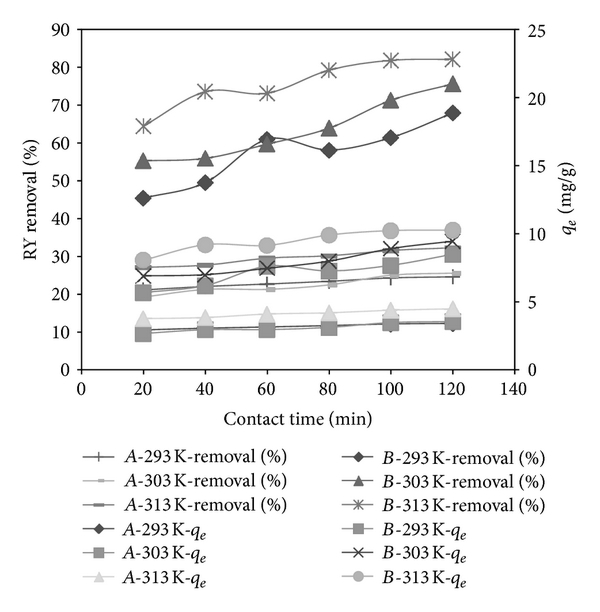
\includegraphics[width=0.35\linewidth]{imagenes/cover} \end{center}

\chapter{Introducción}\label{intro}

Esta unidad tiene por objetivos:

\begin{itemize}
\tightlist
\item
  Entender los principios de los Diseños de Experimentos.
\item
  Reconocer las guías o pautas necesarias de un diseño de experimentos.
\end{itemize}

\section{¿Qué es el método
científico?}\label{que-es-el-metodo-cientifico}

El método científico ha sido el pilar para investigar el mundo natural.
Es a partir de esto que los científicos llegan correctamente a nuevos
conocimientos y actualizan sus conocimientos previos.

De forma general se puede resumir los pasos del método científico como:

\begin{enumerate}
\def\labelenumi{\arabic{enumi}.}
\tightlist
\item
  Observar y realizar una pregunta
\item
  Formular una hipótesis o explicación contrastable.
\item
  Plantear una predición basada en la hipótesis
\item
  Probar la predicciónn.
\item
  Utilizar los resultados para realizar nuevas hipótesis o predicciones.
\end{enumerate}

\subsection*{\texorpdfstring{\emph{ACTIVIDAD}}{ACTIVIDAD}}\label{actividad}
\addcontentsline{toc}{subsection}{\emph{ACTIVIDAD}}

Piense en un fenómeno que desea investigar. Especifique cómo puede
manipular el factor en estudio y mantener todos los demás factores o
condiciones fijas para asegurarse de que estas no influyan en la
respuesta que planea medir.

Luego decida como medir la variable respuesta elegida del factor en
estudio. Si al cambiar los niveles del factor en estudio causa que el
fenómeno cambie, entonces podría concluir que efectivamente existe una
relación de causa y efecto en el trabajo.

\section{¿Estudio de diseño observacional o estudio de diseño
experimental?}\label{estudio-de-diseno-observacional-o-estudio-de-diseno-experimental}

\begin{center}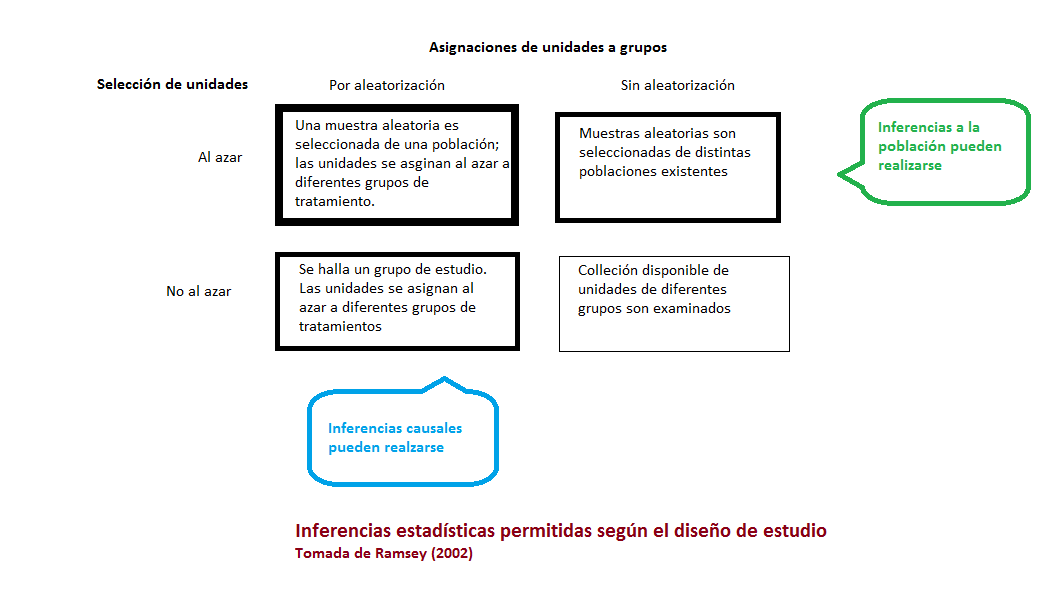
\includegraphics[width=1.5\linewidth]{imagenes/ramsey} \end{center}

\section{Breve historia de los diseño de
experimentos}\label{breve-historia-de-los-diseno-de-experimentos}

\begin{itemize}
\tightlist
\item
  Origen en la agricultura (1918-1940). ANOVA
\item
  Primera era industrial (1951 -- finales 1970). Box \& Wilson.
  Superficies de respuestas. Aplicaciones en procesos químicos e
  industriales
\item
  Segunda era industrial (finales de 1970s -- 1990). Iniciativas de
  mejoramiento de la calidad en algunas compañías. Diseño de Taguchi y
  de parámetros robustos.
\item
  Era moderna. Se caracteriza por emplear técnicas estadísticas para
  tomar decisiones basadas en la calidad. Desarrollo de ensayos
  clínicos.
\end{itemize}

\section{Principios básicos de los diseños
experimentales}\label{principios-basicos-de-los-disenos-experimentales}

\begin{itemize}
\tightlist
\item
  Aleatorización. Componente escencial de cualquier experimento para
  tener validez.
\item
  Replicación. Es fundamental detrás de cada método estadístico para
  saber cuán precisas son las estimaciones finales.
\item
  Control local. Procedimiento para incluir otros factores en un
  experimento que contribuyen a una variación no desaeble. La idea es
  usar creativamente varias técnicas como bloqueo, balanceo, etc para
  controlar las fuentes de variación que reducirán la varianza del
  error.
\end{itemize}

\section{Pasos para planear, conducir y analizar un
experimento}\label{pasos-para-planear-conducir-y-analizar-un-experimento}

Los pasos prácticos necesarios para planificar y realizar un experimento
incluyen: reconocer el objetivo del experimento, elegir los factores,
respuesta(s), diseño, análisis, para luego elaborar conclusiones.

\begin{enumerate}
\def\labelenumi{\arabic{enumi}.}
\tightlist
\item
  Reconocimiento y planteamiento del problema.
\item
  Elección de factores, niveles y rangos.
\item
  Selección de la(s) variable(s) respuesta(s).
\item
  Elección de diseño.
\item
  Conducir el experimento.
\item
  Análisis estadístico.
\item
  Elaborar conclusiones y recomendaciones.
\end{enumerate}

\section{Elementos básicos}\label{elementos-basicos}

\subsection{Unidad experimental}\label{unidad-experimental}

Son elementos o cosas a los cuales se aplica los tratamiento. Pueden ser
personas, ratones, muestras de un material, etc.

\subsection{Error experimental}\label{error-experimental}

Cuantifica la variación existente entre las observaciones tratadas con
iguales tratamientos.

\subsection{Factor}\label{factor}

Variable explicativa o predictora que afecta los resultados del
experimento. Pueden clasificarse de distintos puntos de vista:

\begin{itemize}
\tightlist
\item
  Según sean de interés (factores primarios) o no (ruido).
\item
  Según puedan ser especificado y asignados aleatoriamente: factores
  experimentales y factores de clasificación.
\item
  Factores cualitativos o cuantitativos.
\end{itemize}

Los tratamientos son los niveles de un factor o la combinación de
niveles de los factores de interés.

\textbf{\emph{" To call in the statistician after the experiment is done
may be no more than asking him to perform a post-mortem examination: he
may be able to say what the experiment died of. " (R. Fisher) }}.

\chapter{Experimentos simples
comparativos}\label{experimentos-simples-comparativos}

En esta sesión se tiene como objetivos:

\begin{itemize}
\item
  Revisar los conceptos de estadística básica y herramientas de
  inferencia para experimentos simples comparativos.
\item
  Revisar y probar los supuestos sobre la prueba t
\end{itemize}

\section{Prueba t para dos muestras
independientes}\label{prueba-t-para-dos-muestras-independientes}

Para la prueba t de dos muestras, se supone que ambas muestras provienen
de poblaciones normales con medias \(\mu_i\)(posiblemente diferentes) y
varianzas \(\sigma^2\). Cuando las variazas no son iguales, se puede
intentar superar esto transformando los datos. También existe una
version de la prueba t de dos muestras que puede manejar diferentes
varianzas, pero desafortunadamente esto no se extiende a modelos ANOVA
más complejos. Para probar la hipótesis de que los medias \(\mu_i\) son
iguales: \(H_0:\mu_1 - \mu_2=0\). El Estadístico de prueba es:

\[t_c=\frac{\overline{y}_1-\overline{y}_2}{s_p\sqrt{\frac{1}{n_1}+\frac{1}{n_2}}}\]
\textbf{Nota Sobre el p-valor:} El p-valor es usado como una medida de
credibilidad de la hipótesis. Para la prueba t es la probabilidad de
obtener un valor del estadístico muestral tan extremo o más extremo que
el \(t_c\) en evidencia contra la hipótesis nula, si la hipótesis nula
es correcta

\section{Ejemplo: Motivación y creatividad. Un experimento
aleatorizado}\label{ejemplo-motivacion-y-creatividad.-un-experimento-aleatorizado}

¿Los sistemas de calificación promueven la creatividad en los
estudiantes? ¿Los sistemas de clasificación y los premios de incentivo
aumentan la productividad entre los empleados? ¿Las recompensas y los
elogios estimulan a los niños a aprender? aunque los sistemas de
premiación son profundamente arraigados en la escuela y lugar de
trabajo, cada vez existe más evidencia que sugieren que los premios y
recompensas puede influir de forma opuesta de lo que se espera. Un
estudio memorable fue realizado por la psicóloga Teresa Amabile en un
experimento sobre los efectos de la motivación intrínseca y extrínseca
en la creatividad.\\
(Datos basados en el estudio de Y. Amabile ``Motivation and Creativity:
Effects of Motivational Orientation on Creative Writers''. Journal of
Personality and Social Psychology 48(2) (1985):393-99)

\begin{Shaded}
\begin{Highlighting}[]
\CommentTok{# cargando paquetes y datos:}
\KeywordTok{library}\NormalTok{(Sleuth2)}
\KeywordTok{library}\NormalTok{(mosaic)}
\NormalTok{datos<-case0101}
\KeywordTok{summary}\NormalTok{(datos)}
\end{Highlighting}
\end{Shaded}

\begin{verbatim}
##      Score          Treatment 
##  Min.   : 5.0   Extrinsic:23  
##  1st Qu.:14.9   Intrinsic:24  
##  Median :18.7                 
##  Mean   :17.9                 
##  3rd Qu.:21.2                 
##  Max.   :29.7
\end{verbatim}

\begin{Shaded}
\begin{Highlighting}[]
\KeywordTok{histogram}\NormalTok{(}\OperatorTok{~}\NormalTok{Score }\OperatorTok{|}\StringTok{ }\NormalTok{Treatment, }\DataTypeTok{data =}\NormalTok{ datos)}
\end{Highlighting}
\end{Shaded}

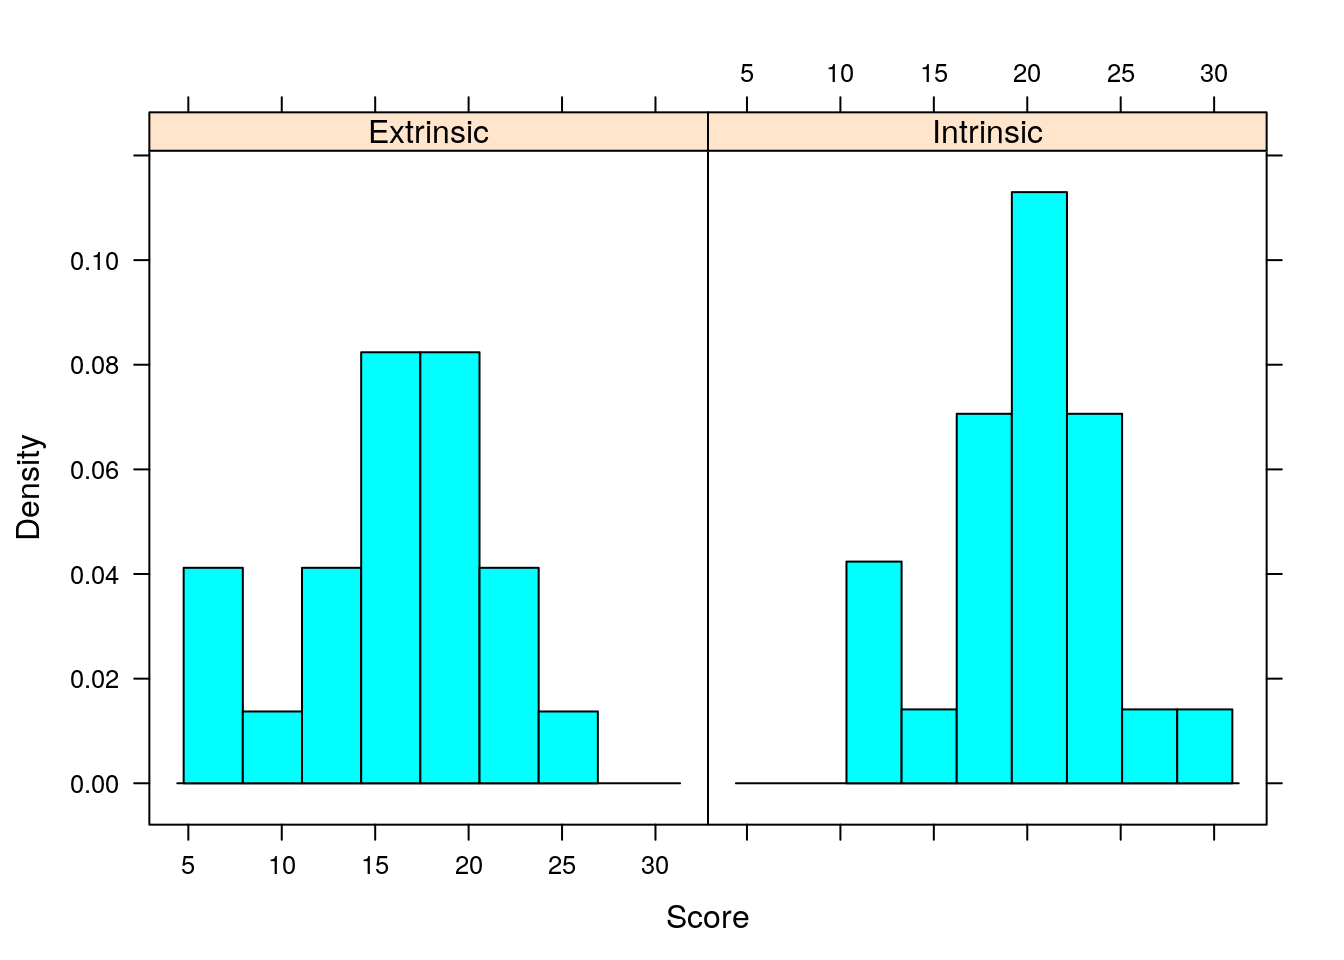
\includegraphics{Introducción_a_los_diseños_experimentales_con_R_files/figure-latex/unnamed-chunk-5-1.pdf}

\begin{Shaded}
\begin{Highlighting}[]
\KeywordTok{plot}\NormalTok{(Score }\OperatorTok{~}\StringTok{ }\NormalTok{Treatment, }\DataTypeTok{data =}\NormalTok{ datos)}
\end{Highlighting}
\end{Shaded}

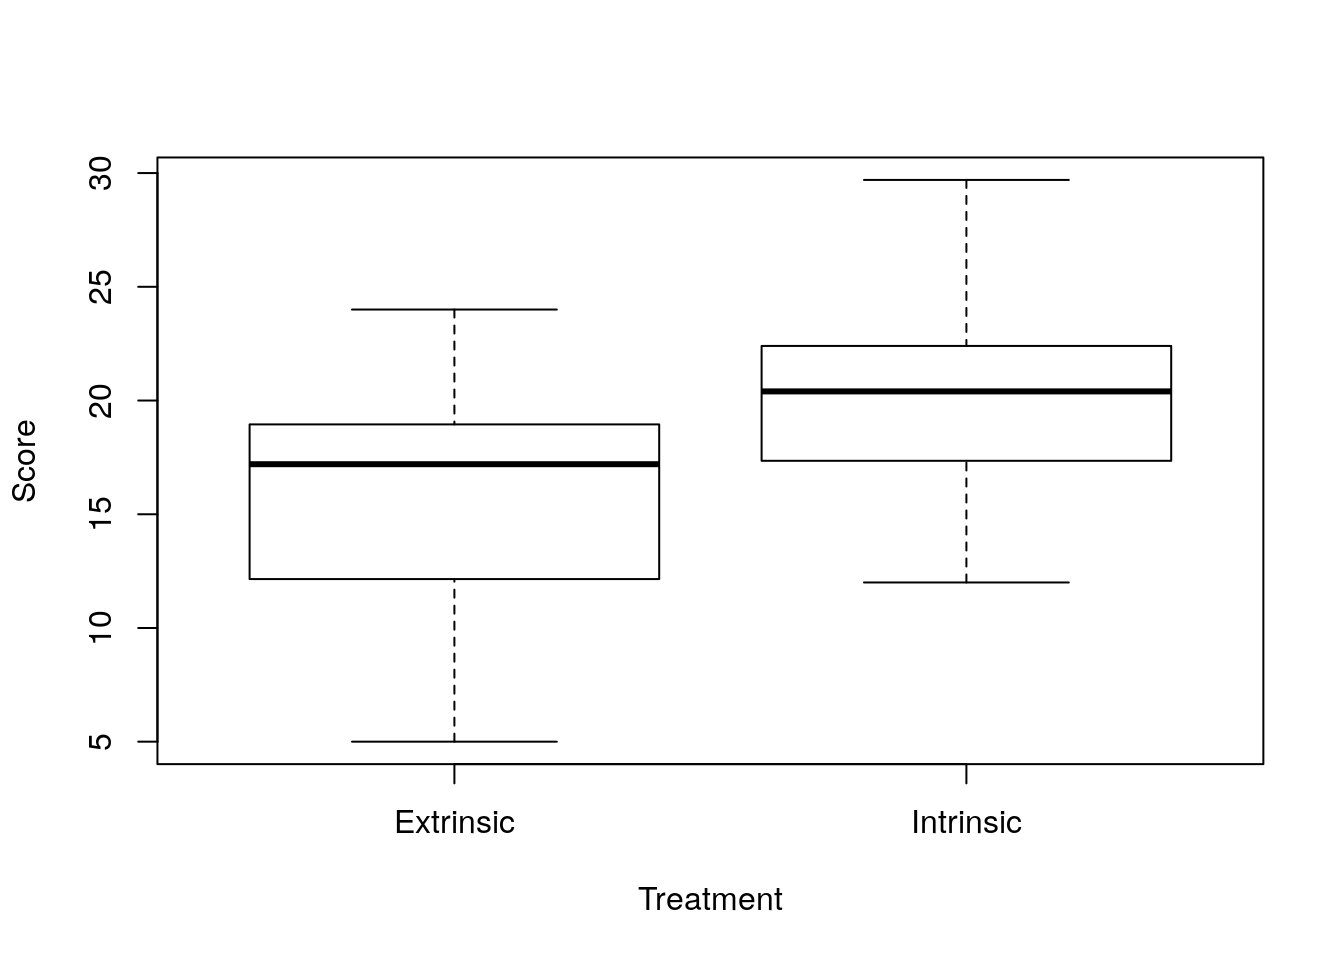
\includegraphics{Introducción_a_los_diseños_experimentales_con_R_files/figure-latex/unnamed-chunk-5-2.pdf}

\begin{Shaded}
\begin{Highlighting}[]
\KeywordTok{favstats}\NormalTok{(Score }\OperatorTok{~}\StringTok{ }\NormalTok{Treatment, }\DataTypeTok{data =}\NormalTok{ datos)}
\end{Highlighting}
\end{Shaded}

\begin{verbatim}
##   Treatment min Q1 median Q3 max mean  sd  n missing
## 1 Extrinsic   5 12     17 19  24   16 5.3 23       0
## 2 Intrinsic  12 17     20 22  30   20 4.4 24       0
\end{verbatim}

\begin{Shaded}
\begin{Highlighting}[]
\KeywordTok{t.test}\NormalTok{(Score }\OperatorTok{~}\StringTok{ }\NormalTok{Treatment, }\DataTypeTok{alternative =} \StringTok{"two.sided"}\NormalTok{, }\DataTypeTok{var.equal =} \OtherTok{TRUE}\NormalTok{, }\DataTypeTok{data =}\NormalTok{ datos)}
\end{Highlighting}
\end{Shaded}

\begin{verbatim}
## 
##  Two Sample t-test
## 
## data:  Score by Treatment
## t = -3, df = 40, p-value = 0.005
## alternative hypothesis: true difference in means is not equal to 0
## 95 percent confidence interval:
##  -7.0 -1.3
## sample estimates:
## mean in group Extrinsic mean in group Intrinsic 
##                      16                      20
\end{verbatim}

\begin{Shaded}
\begin{Highlighting}[]
\KeywordTok{summary}\NormalTok{(}\KeywordTok{lm}\NormalTok{(Score }\OperatorTok{~}\StringTok{ }\NormalTok{Treatment, }\DataTypeTok{data =}\NormalTok{ datos))}
\end{Highlighting}
\end{Shaded}

\begin{verbatim}
## 
## Call:
## lm(formula = Score ~ Treatment, data = datos)
## 
## Residuals:
##    Min     1Q Median     3Q    Max 
## -10.74  -2.98   1.06   2.96   9.82 
## 
## Coefficients:
##             Estimate Std. Error t value Pr(>|t|)    
## (Intercept)   17.811      0.708   25.15   <2e-16 ***
## Treatment1    -2.072      0.708   -2.93   0.0054 ** 
## ---
## Signif. codes:  0 '***' 0.001 '**' 0.01 '*' 0.05 '.' 0.1 ' ' 1
## 
## Residual standard error: 4.8 on 45 degrees of freedom
## Multiple R-squared:  0.16,   Adjusted R-squared:  0.141 
## F-statistic: 8.56 on 1 and 45 DF,  p-value: 0.00537
\end{verbatim}

\begin{Shaded}
\begin{Highlighting}[]
\KeywordTok{anova}\NormalTok{(}\KeywordTok{lm}\NormalTok{(Score }\OperatorTok{~}\StringTok{ }\NormalTok{Treatment, }\DataTypeTok{data =}\NormalTok{ datos))}
\end{Highlighting}
\end{Shaded}

\begin{verbatim}
## Analysis of Variance Table
## 
## Response: Score
##           Df Sum Sq Mean Sq F value Pr(>F)   
## Treatment  1    202   201.7    8.56 0.0054 **
## Residuals 45   1060    23.6                  
## ---
## Signif. codes:  0 '***' 0.001 '**' 0.01 '*' 0.05 '.' 0.1 ' ' 1
\end{verbatim}

\begin{Shaded}
\begin{Highlighting}[]
\NormalTok{residuos<-}\StringTok{ }\KeywordTok{residuals.lm}\NormalTok{(}\KeywordTok{lm}\NormalTok{(Score }\OperatorTok{~}\StringTok{ }\NormalTok{Treatment, }\DataTypeTok{data =}\NormalTok{ datos))}
\NormalTok{datos<-}\KeywordTok{c}\NormalTok{(datos,}\KeywordTok{as.data.frame}\NormalTok{(residuos))}
\KeywordTok{shapiro.test}\NormalTok{(residuos)}
\end{Highlighting}
\end{Shaded}

\begin{verbatim}
## 
##  Shapiro-Wilk normality test
## 
## data:  residuos
## W = 1, p-value = 0.2
\end{verbatim}

\begin{Shaded}
\begin{Highlighting}[]
\KeywordTok{bartlett.test}\NormalTok{(residuos}\OperatorTok{~}\NormalTok{Treatment,datos)}
\end{Highlighting}
\end{Shaded}

\begin{verbatim}
## 
##  Bartlett test of homogeneity of variances
## 
## data:  residuos by Treatment
## Bartlett's K-squared = 0.6, df = 1, p-value = 0.4
\end{verbatim}

\section{Sobre los supuestos:}\label{sobre-los-supuestos}

Los supuestos como muestras independientes provenientes de poblaciones
normales con igual desviación estándar raramente son encontrados en la
práctica. La prueba t de dos muestras es válida a menudo aún si no es
posible asumir estos supuestos debido a su robustes, sin embargo no es
resistente es decir puede ser afectada por pequeños cambios en los datos
(outliers). Es necesario evaluar la adecuación de las herramientas y
decidir usar la prubea estándar o un procedimiento alternativo en cada
problema.

\section{Actividad}\label{actividad-1}

Descargar la data ``Case0301'' de la librería ``Sleuth2''. Los datos que
se muestran fueron recolectados entre 1968 y 1972 para probar la
hipótesis que la inyección masiva de yoduro de plata en cúmulos de nube
puede llevar a un incremento de los niveles de lluvia. En cada uno de
los 52 días que se consideraron adecuados para la siembra de nubes se
deicidió mediante un mecanismo aleatorio sembrar o no (control) la nube
objetivo con yoduro de plata. La precipitación fue medida como el
volumen de lluvia total a lo largo de la trayectoria que siguió el
aeroplano que sobrevoló las nubes.

Realizar un análisis exploratorio con los datos, ¿qué sugieren?

\begin{verbatim}
##     Rainfall       Treatment 
##  Min.   :   1   Unseeded:26  
##  1st Qu.:  29   Seeded  :26  
##  Median : 117                
##  Mean   : 303                
##  3rd Qu.: 307                
##  Max.   :2746
\end{verbatim}

\begin{verbatim}
##   Treatment min Q1 median  Q3  max mean  sd  n missing
## 1  Unseeded 1.0 25     44 159 1203  165 278 26       0
## 2    Seeded 4.1 98    222 406 2746  442 651 26       0
\end{verbatim}

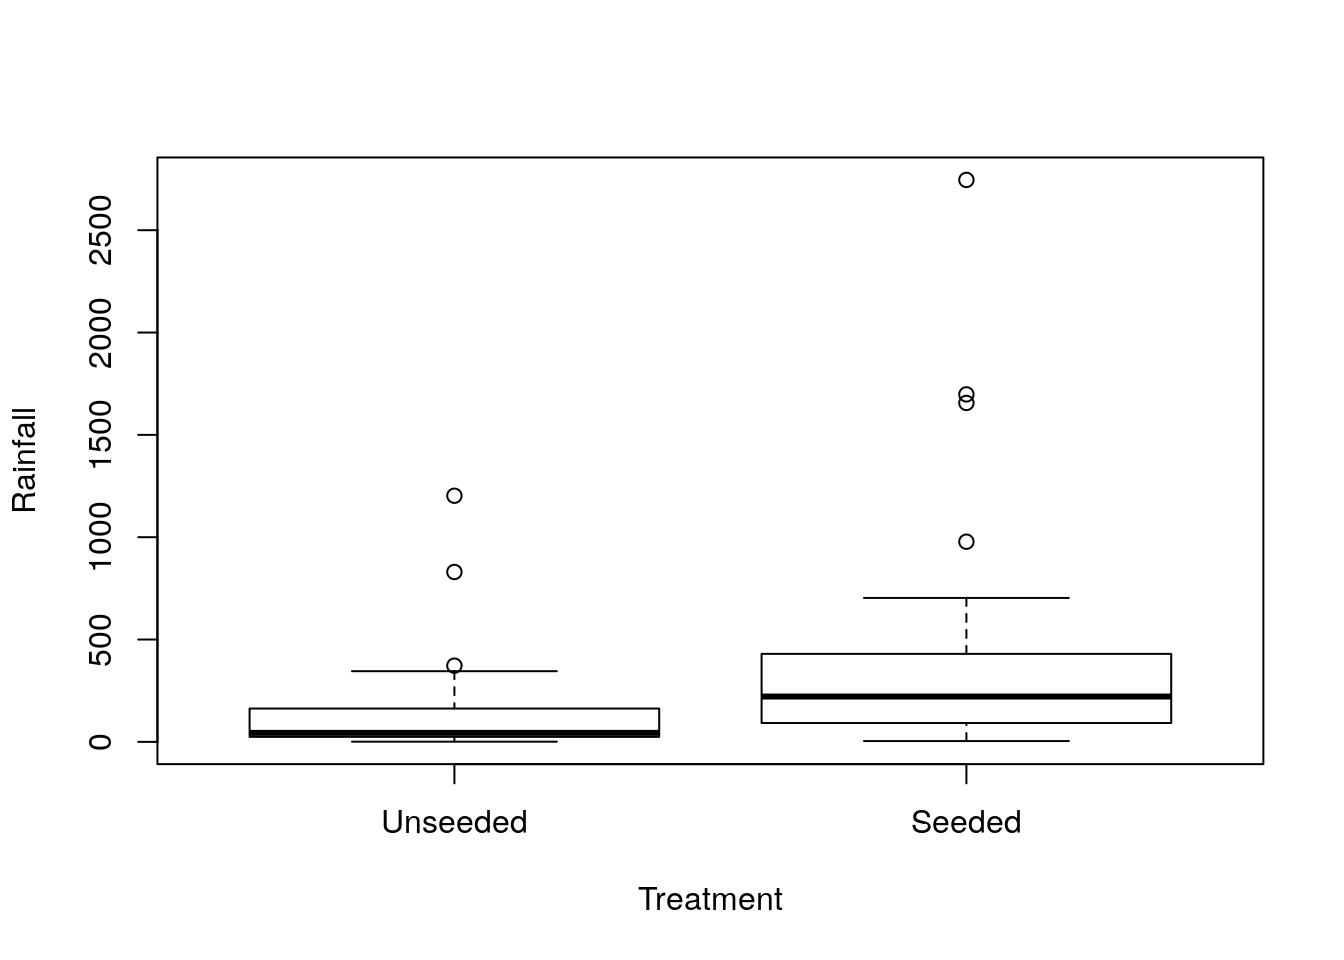
\includegraphics{Introducción_a_los_diseños_experimentales_con_R_files/figure-latex/unnamed-chunk-6-1.pdf}

Realizar un análisis exploratorio con los datos transformado con
logaritmo natural los niveles de lluvia, ¿qué sugieren?

\begin{verbatim}
##   Treatment min  Q1 median  Q3 max mean  sd  n missing
## 1  Unseeded 0.0 3.2    3.8 5.1 7.1  4.0 1.6 26       0
## 2    Seeded 1.4 4.6    5.4 6.0 7.9  5.1 1.6 26       0
\end{verbatim}

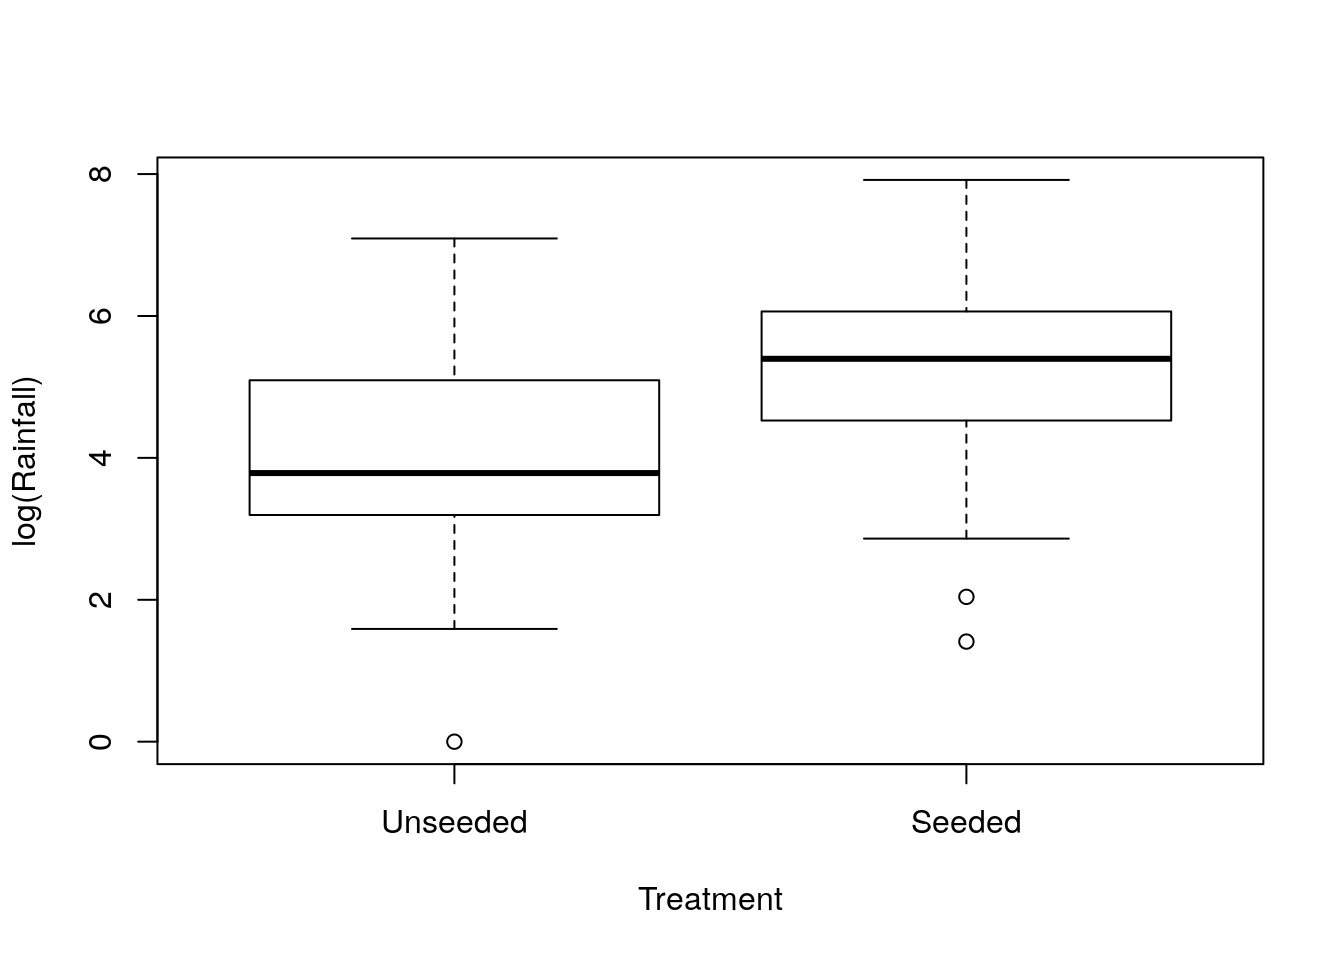
\includegraphics{Introducción_a_los_diseños_experimentales_con_R_files/figure-latex/unnamed-chunk-7-1.pdf}

\begin{verbatim}
## Analysis of Variance Table
## 
## Response: log(Rainfall)
##           Df Sum Sq Mean Sq F value Pr(>F)  
## Treatment  1     17   17.01    6.47  0.014 *
## Residuals 50    131    2.63                 
## ---
## Signif. codes:  0 '***' 0.001 '**' 0.01 '*' 0.05 '.' 0.1 ' ' 1
\end{verbatim}

\begin{verbatim}
## 
## Call:
## lm(formula = log(Rainfall) ~ Treatment, data = datos)
## 
## Residuals:
##    Min     1Q Median     3Q    Max 
## -3.990 -0.745  0.162  1.019  3.102 
## 
## Coefficients:
##             Estimate Std. Error t value Pr(>|t|)    
## (Intercept)    4.562      0.225   20.30   <2e-16 ***
## Treatment1    -0.572      0.225   -2.54    0.014 *  
## ---
## Signif. codes:  0 '***' 0.001 '**' 0.01 '*' 0.05 '.' 0.1 ' ' 1
## 
## Residual standard error: 1.6 on 50 degrees of freedom
## Multiple R-squared:  0.115,  Adjusted R-squared:  0.0969 
## F-statistic: 6.47 on 1 and 50 DF,  p-value: 0.0141
\end{verbatim}

\begin{verbatim}
## Analysis of Variance Table
## 
## Response: Rainfall
##           Df   Sum Sq Mean Sq F value Pr(>F)  
## Treatment  1  1000332 1000332    3.99  0.051 .
## Residuals 50 12526131  250523                 
## ---
## Signif. codes:  0 '***' 0.001 '**' 0.01 '*' 0.05 '.' 0.1 ' ' 1
\end{verbatim}

\chapter{Diseño Completamente al
Azar}\label{diseno-completamente-al-azar}

En esta sección se tiene por objetivos:

\begin{itemize}
\tightlist
\item
  Diseñar un plan para DCA
\item
  Ejecutar el análisis de varianza y evaluación de supuestos
\item
  Realizar pruebas de comparaciones
\end{itemize}

\section{Plan de diseño}\label{plan-de-diseno}

\begin{Shaded}
\begin{Highlighting}[]
\CommentTok{# Cargando paquetes}
\KeywordTok{library}\NormalTok{(agricolae)}
\NormalTok{tratam <-}\StringTok{ }\KeywordTok{c}\NormalTok{(}\StringTok{"A"}\NormalTok{, }\StringTok{"B"}\NormalTok{, }\StringTok{"C"}\NormalTok{)}
\NormalTok{repeticion <-}\StringTok{ }\KeywordTok{c}\NormalTok{(}\DecValTok{4}\NormalTok{, }\DecValTok{3}\NormalTok{, }\DecValTok{4}\NormalTok{)}
\NormalTok{outdesign <-}\StringTok{ }\KeywordTok{design.crd}\NormalTok{(tratam,}\DataTypeTok{r=}\NormalTok{repeticion,}\DataTypeTok{seed=}\DecValTok{777}\NormalTok{,}\DataTypeTok{serie=}\DecValTok{0}\NormalTok{)}
\NormalTok{book1 <-}\StringTok{ }\NormalTok{outdesign}\OperatorTok{$}\NormalTok{book}
\KeywordTok{print}\NormalTok{(book1)}
\end{Highlighting}
\end{Shaded}

\begin{verbatim}
##    plots r tratam
## 1      1 1      B
## 2      2 1      A
## 3      3 2      A
## 4      4 1      C
## 5      5 2      C
## 6      6 3      A
## 7      7 2      B
## 8      8 3      C
## 9      9 3      B
## 10    10 4      A
## 11    11 4      C
\end{verbatim}

\begin{Shaded}
\begin{Highlighting}[]
\KeywordTok{write.csv}\NormalTok{(book1,}\StringTok{"plan1.csv"}\NormalTok{,}\DataTypeTok{row.names=}\OtherTok{FALSE}\NormalTok{)}
\end{Highlighting}
\end{Shaded}

\section{Análisis de Varianza}\label{analisis-de-varianza}

En el diseño experimental de una sola clasificación, o de una sola vía,
las unidades experimentales se considera que provienen de una misma
población, con media \(\mu\), y \(\sigma^2\), luego de la asignación
aleatoria de los \(t\) tratamientos en \(r\) unidades experimentales
cada uno, las unidades experimentales se consideran que provienen de
sub-poblaciones con medía \(\mu_i\) y varianza común \(\sigma^2\),
siendo la media de la i-ésima subpoblación, \(\mu_i=\mu +\tau_i\), igual
a la media general más el efecto del i-ésimo tratamiento \(\tau_i\).

El modelo aditivo lineal: \[y_{ij}=\mu + \tau_i+\epsilon_{ij}\] Las
suposiciones básicas:

\begin{itemize}
\item
  Independencia, las unidades experimentales deben elegirse
  aleatoriamente, las mediciones realizadas en tales unidades
  experimentales deben ser independientes entre sí.
\item
  Homogeneidad de varianzas, las varianzas de las mediciones realizadas
  dentro de cada tratamiento deben ser iguales entre sí, e iguales a una
  varianza común \(\sigma^2\).
\item
  Normalidad, las mediciones deben distribuirse normalmente.
\end{itemize}

Los tratamientos se pueden considerar como:

\begin{itemize}
\item
  Efectos fijos (FIJO), si tan sólo interesa cuantificar los efectos de
  los tratamientos seleccionados para el experimento y comparar entre sí
  tales efectos. El investigador elige los tratamientos a estudiar.
\item
  Efectos al azar (ALEATORIO), si los tratamientos estudiados
  representan una muestra aleatoria de los distintos tratamientos de
  interés para el investigador; interesa conocer la variabilidad
  presente entre los distintos efectos de tratamientos. El investigador
  tiene control parcial sobre qué tratamientos participarán en el
  experimento.
\end{itemize}

Para el Modelo I o de efectos Fijos, la hipótesis a probar es:\\
\(H_0:\mu_1=\mu_2=... =\mu_t=\mu\)\\
\(H_1:\)al menos un \(\mu_i \neq \mu\)

\emph{Ejemplo:}

Un fisiólogo de animales estudió la función pituitaria de las gallinas,
bajo el régimen estándar de muda de pluma forzada que usan los
productores de huevo para mantenerlas en producción. Se usaron 25
gallinas en el estudio. Cinco gallinas se sacrificaron para las
mediciones cada vez, una previa al régimen de muda forzada, y al final
de cada una de las cuatro etapas del régimen. Las cinco condiciones
experimentales (tratamientos) corresponden a: 1) premuda (control), 2)
ayuno de 8 días, 3) 60 gramos de salvado al día durante 10 días, 4) 80
gramos de salvado al día durante 10 días y 5) mezcla de malta durante 42
días. El objetivo era monitorear las respuestas fisiológicas asociadas
con la función pituitaria de las gallinas durante el régimen para
explicar por qué vuelven a producir después de la muda forzada. Uno de
los compuestos medidos fue la concentración de suero T3. Los datos de la
tabla son las medidas de suero T3 en las cinco gallinas sacrificadas al
final de cada etapa del régimen.\\
(Ejercicio 2.3 tomado del libro Diseños de Experimentos de R. Kuehl)

\begin{Shaded}
\begin{Highlighting}[]
\CommentTok{# Cargando datos:}
\KeywordTok{library}\NormalTok{(mosaic)}
\NormalTok{datos <-}\StringTok{ }\KeywordTok{read.table}\NormalTok{(}\StringTok{"kuehl2.3.txt"}\NormalTok{,}\DataTypeTok{header=}\NormalTok{T)}
\KeywordTok{summary}\NormalTok{(datos)}
\end{Highlighting}
\end{Shaded}

\begin{verbatim}
##       trat      serum.T3  
##  Min.   :1   Min.   : 74  
##  1st Qu.:2   1st Qu.: 90  
##  Median :3   Median :103  
##  Mean   :3   Mean   :121  
##  3rd Qu.:4   3rd Qu.:120  
##  Max.   :5   Max.   :226
\end{verbatim}

\begin{Shaded}
\begin{Highlighting}[]
\KeywordTok{favstats}\NormalTok{(serum.T3 }\OperatorTok{~}\StringTok{ }\NormalTok{trat, }\DataTypeTok{data =}\NormalTok{ datos)}
\end{Highlighting}
\end{Shaded}

\begin{verbatim}
##   trat min  Q1 median  Q3 max mean   sd n missing
## 1    1  74  74     90  94  99   86 11.8 5       0
## 2    2  99 104    115 118 129  113 12.0 5       0
## 3    3 178 197    207 223 226  206 19.8 5       0
## 4    4 101 103    112 118 120  111  8.5 5       0
## 5    5  83  83     88  90  96   88  5.5 5       0
\end{verbatim}

\begin{Shaded}
\begin{Highlighting}[]
\NormalTok{datos}\OperatorTok{$}\NormalTok{trat<-}\KeywordTok{as.factor}\NormalTok{(datos}\OperatorTok{$}\NormalTok{trat)}
\KeywordTok{anova}\NormalTok{(}\KeywordTok{lm}\NormalTok{(serum.T3}\OperatorTok{~}\NormalTok{trat,datos))}
\end{Highlighting}
\end{Shaded}

\begin{verbatim}
## Analysis of Variance Table
## 
## Response: serum.T3
##           Df Sum Sq Mean Sq F value  Pr(>F)    
## trat       4  48569   12142    78.1 6.5e-12 ***
## Residuals 20   3110     156                    
## ---
## Signif. codes:  0 '***' 0.001 '**' 0.01 '*' 0.05 '.' 0.1 ' ' 1
\end{verbatim}

\begin{Shaded}
\begin{Highlighting}[]
\KeywordTok{summary}\NormalTok{(}\KeywordTok{lm}\NormalTok{(serum.T3}\OperatorTok{~}\NormalTok{trat,datos))}
\end{Highlighting}
\end{Shaded}

\begin{verbatim}
## 
## Call:
## lm(formula = serum.T3 ~ trat, data = datos)
## 
## Residuals:
##    Min     1Q Median     3Q    Max 
## -28.66  -8.98   1.32   7.72  19.89 
## 
## Coefficients:
##             Estimate Std. Error t value Pr(>|t|)    
## (Intercept)   120.81       2.49   48.44  < 2e-16 ***
## trat1         -34.44       4.99   -6.90  1.1e-06 ***
## trat2          -7.96       4.99   -1.60    0.126    
## trat3          85.35       4.99   17.11  2.1e-13 ***
## trat4         -10.12       4.99   -2.03    0.056 .  
## ---
## Signif. codes:  0 '***' 0.001 '**' 0.01 '*' 0.05 '.' 0.1 ' ' 1
## 
## Residual standard error: 12 on 20 degrees of freedom
## Multiple R-squared:  0.94,   Adjusted R-squared:  0.928 
## F-statistic: 78.1 on 4 and 20 DF,  p-value: 6.48e-12
\end{verbatim}

\begin{Shaded}
\begin{Highlighting}[]
\KeywordTok{par}\NormalTok{(}\DataTypeTok{mfrow=}\KeywordTok{c}\NormalTok{(}\DecValTok{2}\NormalTok{,}\DecValTok{2}\NormalTok{))}
\KeywordTok{plot}\NormalTok{(}\KeywordTok{lm}\NormalTok{(serum.T3}\OperatorTok{~}\NormalTok{trat,datos))}
\end{Highlighting}
\end{Shaded}

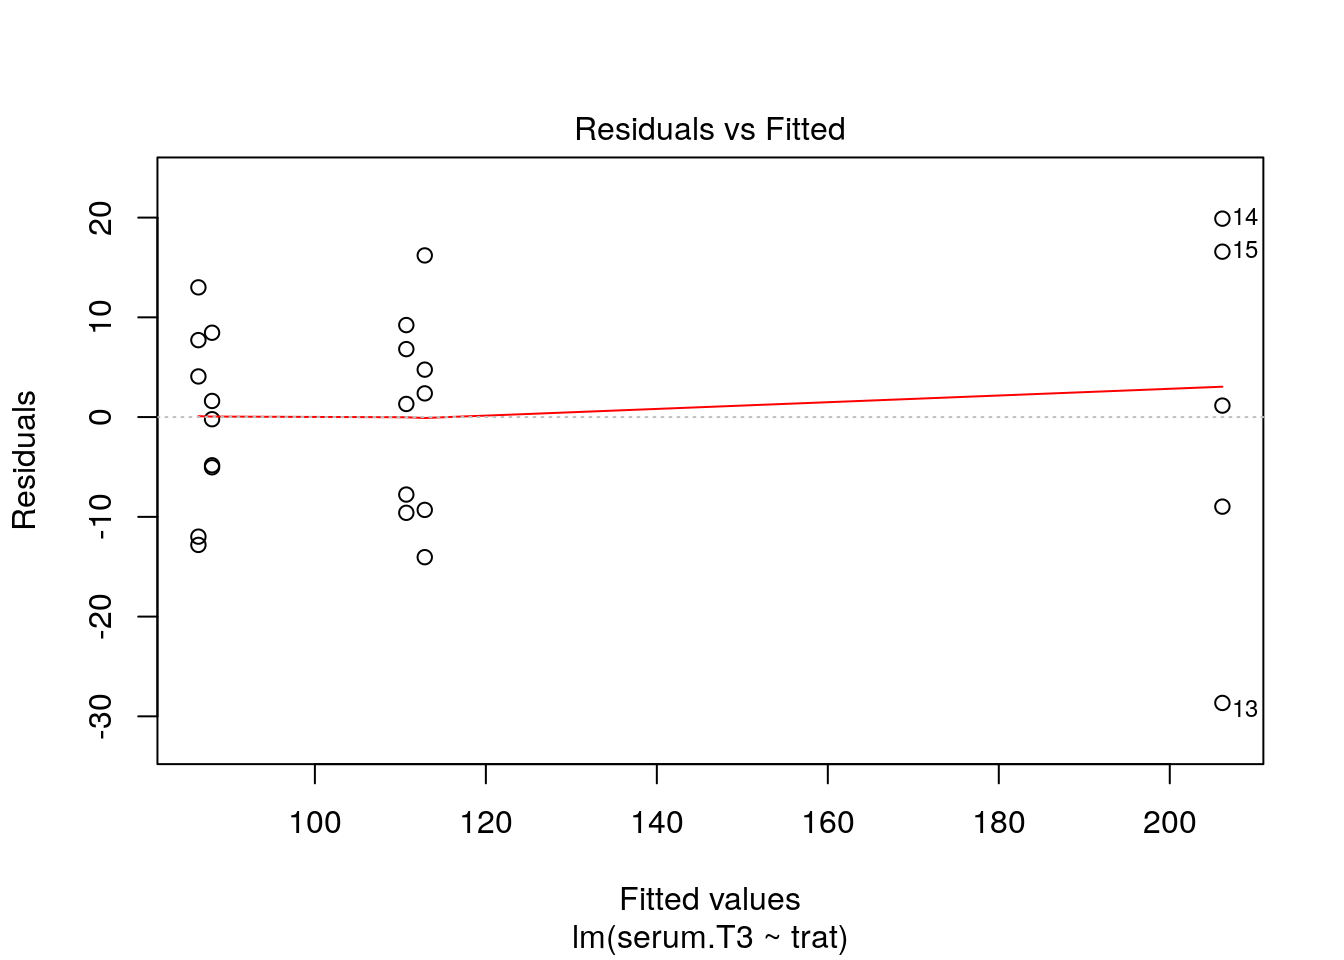
\includegraphics{Introducción_a_los_diseños_experimentales_con_R_files/figure-latex/unnamed-chunk-10-1.pdf}

\begin{Shaded}
\begin{Highlighting}[]
\NormalTok{residuales<-}\KeywordTok{residuals}\NormalTok{(}\KeywordTok{lm}\NormalTok{(serum.T3}\OperatorTok{~}\NormalTok{trat,datos))}
\NormalTok{datos<-}\KeywordTok{cbind}\NormalTok{(datos,}\KeywordTok{as.data.frame}\NormalTok{(residuales))}
\KeywordTok{library}\NormalTok{(nortest)}
\KeywordTok{ad.test}\NormalTok{(residuales)}
\end{Highlighting}
\end{Shaded}

\begin{verbatim}
## 
##  Anderson-Darling normality test
## 
## data:  residuales
## A = 0.2, p-value = 0.8
\end{verbatim}

\begin{Shaded}
\begin{Highlighting}[]
\CommentTok{#library(car)}
\CommentTok{#leveneTest(serum.T3~trat,datos)}
\end{Highlighting}
\end{Shaded}

\section{Prueba de Comparaciones por
pares}\label{prueba-de-comparaciones-por-pares}

\begin{Shaded}
\begin{Highlighting}[]
\KeywordTok{pairwise.t.test}\NormalTok{(datos}\OperatorTok{$}\NormalTok{serum.T3,datos}\OperatorTok{$}\NormalTok{trat,}\DataTypeTok{p.adjust.method=}\StringTok{"none"}\NormalTok{)}
\end{Highlighting}
\end{Shaded}

\begin{verbatim}
## 
##  Pairwise comparisons using t tests with pooled SD 
## 
## data:  datos$serum.T3 and datos$trat 
## 
##   1     2     3     4    
## 2 0.003 -     -     -    
## 3 2e-12 2e-10 -     -    
## 4 0.006 0.787 1e-10 -    
## 5 0.841 0.005 2e-12 0.009
## 
## P value adjustment method: none
\end{verbatim}

\section{Prueba de comparaciones
Múltiples}\label{prueba-de-comparaciones-multiples}

Buscan controlar la probabilidad de cometer el error Tipo I a nivel del
experimento, cuando se realizan comparaciones entre las medias de tres o
más tratamientos. Entre las procedimientos de comparaciones múltiples
tenemos:

\subsection{Diferencia Mínima
Significativa(DLS)}\label{diferencia-minima-significativadls}

Se basa en la prueba de t para pares de medias. Se recomienda realizar
la prueba tan sólo si la prueba F del Análisis de Varianza resulta
significativa. Si el número de comparaciones es muy grande se recomienda
utilizar la corrección de Bonferroni y utilizar el nivel de
significación \(\alpha/k\), donde \(k=\frac{t(t-1)}{2}\); de esta
manera, el nivel de significación del conjunto de comparaciones (nivel
de significación del experimento) es \(\alpha\).

\begin{Shaded}
\begin{Highlighting}[]
\KeywordTok{pairwise.t.test}\NormalTok{(datos}\OperatorTok{$}\NormalTok{serum.T3,datos}\OperatorTok{$}\NormalTok{trat, }\DataTypeTok{p.adjust.method =} \StringTok{"bonf"}\NormalTok{)}
\end{Highlighting}
\end{Shaded}

\begin{verbatim}
## 
##  Pairwise comparisons using t tests with pooled SD 
## 
## data:  datos$serum.T3 and datos$trat 
## 
##   1     2     3     4   
## 2 0.03  -     -     -   
## 3 2e-11 2e-09 -     -   
## 4 0.06  1.00  1e-09 -   
## 5 1.00  0.05  2e-11 0.09
## 
## P value adjustment method: bonferroni
\end{verbatim}

\subsection{\texorpdfstring{Prueba de Tukey para \emph{post-hoc}
comparaciones de pares de
tratamientos}{Prueba de Tukey para post-hoc comparaciones de pares de tratamientos}}\label{prueba-de-tukey-para-post-hoc-comparaciones-de-pares-de-tratamientos}

Se basa en la diferencia estudiantizada, para probar la hipótesis nula
\(H_0:\mu_i=\mu_j\) versus la alternativa hipótesis
\(H_0:\mu_i\neq\mu_j\) ,para todo \(i,j=1,2,...t\), a un nivel de
significación \(\alpha\) se le conoce como prueba de la Diferencia
Honestamente Significativa (DHS), ejerce control sobre el nivel de
significación del experimento cuando el número de repeticiones es el
mismo en cada tratamiento. Esta prueba requiere que las medias de los
tratamientos no estén correlacionadas y tengan igual varianzas, es
decir, el número de repeticiones de cada tratamiento debe ser el mismo.
Mantiene el nivel de significación del experimento al nivel determinado,
pero en cambio resulta con menor potencia, siendo una prueba de
significación conservadora.

\begin{Shaded}
\begin{Highlighting}[]
\KeywordTok{TukeyHSD}\NormalTok{(}\KeywordTok{aov}\NormalTok{(serum.T3}\OperatorTok{~}\NormalTok{trat,datos))}
\end{Highlighting}
\end{Shaded}

\begin{verbatim}
##   Tukey multiple comparisons of means
##     95% family-wise confidence level
## 
## Fit: aov(formula = serum.T3 ~ trat, data = datos)
## 
## $trat
##       diff     lwr    upr p adj
## 2-1   26.5    2.88  50.08  0.02
## 3-1  119.8   96.18 143.38  0.00
## 4-1   24.3    0.72  47.92  0.04
## 5-1    1.6  -22.00  25.20  1.00
## 3-2   93.3   69.70 116.90  0.00
## 4-2   -2.2  -25.76  21.44  1.00
## 5-2  -24.9  -48.48  -1.28  0.04
## 4-3  -95.5 -119.06 -71.86  0.00
## 5-3 -118.2 -141.78 -94.58  0.00
## 5-4  -22.7  -46.32   0.88  0.06
\end{verbatim}

\begin{Shaded}
\begin{Highlighting}[]
\KeywordTok{library}\NormalTok{(multcomp)}
\NormalTok{model<-}\KeywordTok{aov}\NormalTok{(}\DataTypeTok{formula =}\NormalTok{ serum.T3 }\OperatorTok{~}\StringTok{ }\NormalTok{trat, }\DataTypeTok{data =}\NormalTok{ datos)}
\NormalTok{compTukey<-}\StringTok{ }\KeywordTok{confint}\NormalTok{(}\KeywordTok{glht}\NormalTok{(model, }\DataTypeTok{linfct =} \KeywordTok{mcp}\NormalTok{(}\DataTypeTok{trat =} \StringTok{"Tukey"}\NormalTok{)))}
\KeywordTok{summary}\NormalTok{(compTukey)}
\end{Highlighting}
\end{Shaded}

\begin{verbatim}
## 
##   Simultaneous Tests for General Linear Hypotheses
## 
## Multiple Comparisons of Means: Tukey Contrasts
## 
## 
## Fit: aov(formula = serum.T3 ~ trat, data = datos)
## 
## Linear Hypotheses:
##            Estimate Std. Error t value Pr(>|t|)    
## 2 - 1 == 0    26.48       7.89    3.36    0.023 *  
## 3 - 1 == 0   119.78       7.89   15.19   <0.001 ***
## 4 - 1 == 0    24.32       7.89    3.08    0.041 *  
## 5 - 1 == 0     1.60       7.89    0.20    1.000    
## 3 - 2 == 0    93.30       7.89   11.83   <0.001 ***
## 4 - 2 == 0    -2.16       7.89   -0.27    0.999    
## 5 - 2 == 0   -24.88       7.89   -3.15    0.036 *  
## 4 - 3 == 0   -95.46       7.89  -12.10   <0.001 ***
## 5 - 3 == 0  -118.18       7.89  -14.98   <0.001 ***
## 5 - 4 == 0   -22.72       7.89   -2.88    0.063 .  
## ---
## Signif. codes:  0 '***' 0.001 '**' 0.01 '*' 0.05 '.' 0.1 ' ' 1
## (Adjusted p values reported -- single-step method)
\end{verbatim}

\subsection{Prueba de Dunnett para comparar cada uno de los tratamientos
a un
control}\label{prueba-de-dunnett-para-comparar-cada-uno-de-los-tratamientos-a-un-control}

Se utiliza cuando las comparaciones de interés (a priori) son entre un
conjunto de (t--1) medias de tratamientos no correlacionadas y un
control. Se obtiene mayor potencia mediante el uso de un método de
comparación que se restringe a comparar cada tratamiento con el control.
La prueba de Dunnett controla el Error Tipo I de las comparaciones
individuales y mantiene el nivel de significación del experimento al
nivel \(\alpha\) determinado.

En el ejemplo asumiendo que premuda es el control

\begin{Shaded}
\begin{Highlighting}[]
\KeywordTok{library}\NormalTok{(multcomp)}
\NormalTok{ni<-}\KeywordTok{tapply}\NormalTok{(datos}\OperatorTok{$}\NormalTok{serum.T3,datos}\OperatorTok{$}\NormalTok{trat,length)}
\NormalTok{contr<-}\KeywordTok{contrMat}\NormalTok{(ni,}\DataTypeTok{type=}\StringTok{"Dunnet"}\NormalTok{)}
\NormalTok{model<-}\KeywordTok{aov}\NormalTok{(}\DataTypeTok{formula =}\NormalTok{ serum.T3 }\OperatorTok{~}\StringTok{ }\NormalTok{trat, }\DataTypeTok{data =}\NormalTok{ datos)}
\NormalTok{compDunnet<-}\StringTok{ }\KeywordTok{confint}\NormalTok{ (}\KeywordTok{glht}\NormalTok{(model, }\DataTypeTok{linfct =} \KeywordTok{mcp}\NormalTok{(}\DataTypeTok{trat =}\NormalTok{ contr)))}
\NormalTok{compDunnet}
\end{Highlighting}
\end{Shaded}

\begin{verbatim}
## 
##   Simultaneous Confidence Intervals
## 
## Multiple Comparisons of Means: User-defined Contrasts
## 
## 
## Fit: aov(formula = serum.T3 ~ trat, data = datos)
## 
## Quantile = 2.6
## 95% family-wise confidence level
##  
## 
## Linear Hypotheses:
##            Estimate lwr     upr    
## 2 - 1 == 0  26.478    5.584  47.372
## 3 - 1 == 0 119.782   98.888 140.676
## 4 - 1 == 0  24.320    3.426  45.214
## 5 - 1 == 0   1.598  -19.296  22.492
\end{verbatim}

\begin{Shaded}
\begin{Highlighting}[]
\KeywordTok{summary}\NormalTok{(compDunnet)}
\end{Highlighting}
\end{Shaded}

\begin{verbatim}
## 
##   Simultaneous Tests for General Linear Hypotheses
## 
## Multiple Comparisons of Means: User-defined Contrasts
## 
## 
## Fit: aov(formula = serum.T3 ~ trat, data = datos)
## 
## Linear Hypotheses:
##            Estimate Std. Error t value Pr(>|t|)    
## 2 - 1 == 0    26.48       7.89    3.36    0.011 *  
## 3 - 1 == 0   119.78       7.89   15.19   <0.001 ***
## 4 - 1 == 0    24.32       7.89    3.08    0.020 *  
## 5 - 1 == 0     1.60       7.89    0.20    0.999    
## ---
## Signif. codes:  0 '***' 0.001 '**' 0.01 '*' 0.05 '.' 0.1 ' ' 1
## (Adjusted p values reported -- single-step method)
\end{verbatim}

\subsection{Pruebas de Duncan}\label{pruebas-de-duncan}

El contraste de Duncan utiliza, como el HSD de Tukey, la distribución
del recorrido estudentizado. Se diferencia de ese test en que su
aplicación es secuencial, en el sentido de no utilizar un único valor
crítico para todas las diferencias de medias, como el de Tukey, sino un
valor crítico que depende del número de medias comprendido entre las dos
medias que se comparan, habiendo ordenado previamente las medias en
orden creciente.

\begin{Shaded}
\begin{Highlighting}[]
\KeywordTok{library}\NormalTok{(agricolae)}
\NormalTok{model<-}\KeywordTok{aov}\NormalTok{(}\DataTypeTok{formula =}\NormalTok{ serum.T3 }\OperatorTok{~}\StringTok{ }\NormalTok{trat, }\DataTypeTok{data =}\NormalTok{ datos)}
\KeywordTok{duncan.test}\NormalTok{(model,}\StringTok{"trat"}\NormalTok{,}\DataTypeTok{console=}\OtherTok{TRUE}\NormalTok{)}
\end{Highlighting}
\end{Shaded}

\begin{verbatim}
## 
## Study: model ~ "trat"
## 
## Duncan's new multiple range test
## for serum.T3 
## 
## Mean Square Error:  156 
## 
## trat,  means
## 
##   serum.T3  std r Min Max
## 1       86 11.8 5  74  99
## 2      113 12.0 5  99 129
## 3      206 19.8 5 178 226
## 4      111  8.5 5 101 120
## 5       88  5.5 5  83  96
## 
## Alpha: 0.05 ; DF Error: 20 
## 
## Critical Range
##  2  3  4  5 
## 16 17 18 18 
## 
## Means with the same letter are not significantly different.
## 
##   serum.T3 groups
## 3      206      a
## 2      113      b
## 4      111      b
## 5       88      c
## 1       86      c
\end{verbatim}

\subsection{Pruebas de significación de contrastes para comparaciones
pre-planeadas}\label{pruebas-de-significacion-de-contrastes-para-comparaciones-pre-planeadas}

Al planear un experimento, los tratamientos se seleccionan de tal manera
que comparaciones entre ellos permitan responder a las interrogantes que
suscitaron la realización del experimento. Estas comparaciones
pre-planeadas se pueden analizar mediante contrastes. Un contraste
corresponde a una función lineal de las medias de tratamientos, definida
por una determinada comparación de interés.
\[C=\sum_{i=1}^{t}{C_i\mu_i}\] tal que: \(\sum{c_i=0}\) para el caso
balanceado.\\
Se puede utilizar una prueba de F para probar la hipótesis nula de que
el contraste \(C\) es igual a cero, \(H_0: C = 0\) versus la hipótesis
alternativa \(H_1:C\neq0\) a un nivel de significación \(\alpha\).

En el ejemplo suponga que se quiere probar smultáneamente:\\
\[H_0:\mu_1=\mu_3
\\ \mu_1+\mu_3 =\mu_4+\mu_5
\\ \mu_4=\mu_5
\\ 4\mu_2=\mu_1+\mu_3+\mu_4+\mu_5\]

\begin{Shaded}
\begin{Highlighting}[]
\KeywordTok{library}\NormalTok{(multcomp)}
\NormalTok{model<-}\KeywordTok{aov}\NormalTok{(}\DataTypeTok{formula =}\NormalTok{ serum.T3 }\OperatorTok{~}\StringTok{ }\NormalTok{trat, }\DataTypeTok{data =}\NormalTok{ datos)}
\NormalTok{K <-}\StringTok{ }\KeywordTok{rbind}\NormalTok{(}\StringTok{"1 vs 3"}\NormalTok{ =}\StringTok{ }\KeywordTok{c}\NormalTok{(}\DecValTok{1}\NormalTok{,}\DecValTok{0}\NormalTok{,}\OperatorTok{-}\DecValTok{1}\NormalTok{,}\DecValTok{0}\NormalTok{,}\DecValTok{0}\NormalTok{),}
\StringTok{"1,3 vs 4,5"}\NormalTok{ =}\StringTok{ }\KeywordTok{c}\NormalTok{(}\OperatorTok{-}\DecValTok{1}\NormalTok{,}\DecValTok{0}\NormalTok{,}\OperatorTok{-}\DecValTok{1}\NormalTok{,}\DecValTok{1}\NormalTok{,}\DecValTok{1}\NormalTok{),}
\StringTok{"4 vs 5"}\NormalTok{ =}\StringTok{ }\KeywordTok{c}\NormalTok{(}\DecValTok{0}\NormalTok{,}\DecValTok{0}\NormalTok{,}\DecValTok{0}\NormalTok{,}\DecValTok{1}\NormalTok{,}\OperatorTok{-}\DecValTok{1}\NormalTok{),}
\StringTok{"2 vs 1,3,4,5"}\NormalTok{ =}\StringTok{ }\KeywordTok{c}\NormalTok{(}\OperatorTok{-}\DecValTok{1}\NormalTok{,}\DecValTok{4}\NormalTok{,}\OperatorTok{-}\DecValTok{1}\NormalTok{,}\OperatorTok{-}\DecValTok{1}\NormalTok{,}\OperatorTok{-}\DecValTok{1}\NormalTok{))}
\NormalTok{comp <-}\StringTok{ }\KeywordTok{glht}\NormalTok{(model,}\DataTypeTok{linfct =} \KeywordTok{mcp}\NormalTok{(}\DataTypeTok{trat=}\NormalTok{K),}\DataTypeTok{alternative =} \StringTok{"two.sided"}\NormalTok{)}
\KeywordTok{summary}\NormalTok{(comp)}
\end{Highlighting}
\end{Shaded}

\begin{verbatim}
## 
##   Simultaneous Tests for General Linear Hypotheses
## 
## Multiple Comparisons of Means: User-defined Contrasts
## 
## 
## Fit: aov(formula = serum.T3 ~ trat, data = datos)
## 
## Linear Hypotheses:
##                   Estimate Std. Error t value Pr(>|t|)    
## 1 vs 3 == 0        -119.78       7.89  -15.19   <0.001 ***
## 1,3 vs 4,5 == 0     -93.86      11.15   -8.42   <0.001 ***
## 4 vs 5 == 0          22.72       7.89    2.88    0.036 *  
## 2 vs 1,3,4,5 == 0   -39.79      24.94   -1.60    0.401    
## ---
## Signif. codes:  0 '***' 0.001 '**' 0.01 '*' 0.05 '.' 0.1 ' ' 1
## (Adjusted p values reported -- single-step method)
\end{verbatim}

\section{Actividad}\label{actividad-2}

Una serie de estudios, que involucran varias especies de animales,
hallaron que la restricción de ingesta calórica puede incrementar
dramáticamente la esperanza de vida. En uno de tales estudios en ratones
hembras fueron asignados aleatoriamente a uno de los seis grupos de
tratamientos siguientes:

\begin{itemize}
\tightlist
\item
  Grupo NP: los ratones comían tanto como quisiera de una dieta estándar
  de laboratorio.
\item
  Grupo N/N85: este grupo fue alimentado normalmente antes y después del
  destete. Después del destete la ración fue controlada a 85kcl/wk. Este
  grupo además del grupo NP, sirve como control pues la ingesta de
  calorías es razonablemente constante.
\item
  Grupo N/R50: este grupo fue alimentado con una dieta normal antes del
  destete y una dieta reducida en calorías de 50 kcal/wk después del
  destete.
\item
  Grupo R/R50: este grupo fue alimentado con una dieta reducida en
  calorías de 50 kcal/wk antes y después del destete.
\item
  Grupo N/R50 lopro: este grupo fue alimentado con una dieta normal
  antes del destete, con una dieta reducida en calorías de 50 kcal/wk
  después del destete y con un contenido proteico que disminuía con la
  edad.
\item
  Grupo N/R40: este grupo fue alimentado con una dieta normal antes del
  destete y con una dieta drásticamente reducida en calorías de 40
  kcal/wk después del destete
\end{itemize}

Los datos (case0501) se descargan desde la librería ``Sleuth2''.

Realice el análisis correspondientes

\chapter{Diseño en Bloque Completamente al
Azar}\label{diseno-en-bloque-completamente-al-azar}

En esta sección se tiene por objetivos:

\begin{itemize}
\tightlist
\item
  Diseñar un plan para DCA
\item
  Ejecutar el análisis de varianza y evaluación de supuestos
\item
  Realizar pruebas de comparaciones
\end{itemize}

Este diseño se caracteriza por la presencia de un factor de variación
conocido entre las unidades experimentales, lo cual nos lleva a agrupar
las unidades experimentales en grupos homogéneos o bloques. Los
tratamientos se asignan aleatoriamente a las unidades experimentales de
cada bloque. Todos los tratamientos están presentes en cada uno de los
bloques (bloques completos). El número de unidades experimentales dentro
de cada bloque es igual al número de tratamientos. Se tiene una
observación por tratamiento dentro de cada bloque (diseño es
balanceado). No es posible medir la interacción Bloques \(\times\)
Tratamiento, la cual se supone no es significativa; en caso contrario,
se recomienda no utilizar este diseño. El factor de bloqueo se considera
como una fuente de variación conocida que genera cierta patrón de
respuesta en los tratamientos aplicados en el mismo bloque y que explica
una porción de la variabilidad observada entre unidades experimentales
sometidas al mismo tratamiento, la otra porción se considera producto de
la variación natural debido a efectos aleatorios de origen desconocido.
Si se ignorase la presencia de la fuente de variabilidad conocida
(Bloques) y se condujese el experimento con un diseño completamente al
azar, tendríamos que el Error Experimental para DCA comprendería la
variación debido al factor de bloque más la variación natural debido a
efectos aleatorios no controlados. Las pruebas de significación serían
erradas ya que el Cuadrado Medio del Error sería mayor del debido.

Suposiciones Básicas del Diseño:

\begin{itemize}
\tightlist
\item
  Independencia de las unidades experimentales dentro de cada bloque y
  entre bloques
\item
  Homogeneidad de las varianzas dentro de cada tratamiento
\item
  Normalidad de los errores
\item
  El efecto de interacción Bloque \(\times\) Tratamiento no existe o es
  despreciable
\item
  Aditividad de efectos de Bloques y Tratamientos
\end{itemize}

\section{Plan de diseño}\label{plan-de-diseno-1}

\begin{Shaded}
\begin{Highlighting}[]
\CommentTok{# Cargando paquetes}
\KeywordTok{library}\NormalTok{(agricolae)}
\NormalTok{trt <-}\StringTok{ }\KeywordTok{c}\NormalTok{(}\StringTok{"A"}\NormalTok{, }\StringTok{"B"}\NormalTok{, }\StringTok{"C"}\NormalTok{,}\StringTok{"D"}\NormalTok{,}\StringTok{"E"}\NormalTok{)}
\NormalTok{repeticion <-}\StringTok{ }\DecValTok{4}
\NormalTok{outdesign <-}\StringTok{ }\KeywordTok{design.rcbd}\NormalTok{(trt,}\DataTypeTok{r=}\NormalTok{repeticion, }\DataTypeTok{seed=}\OperatorTok{-}\DecValTok{513}\NormalTok{, }\DataTypeTok{serie=}\DecValTok{1}\NormalTok{)}
\NormalTok{book2 <-}\StringTok{ }\NormalTok{outdesign}\OperatorTok{$}\NormalTok{book}
\KeywordTok{print}\NormalTok{(book2)}
\end{Highlighting}
\end{Shaded}

\begin{verbatim}
##    plots block trt
## 1     11     1   D
## 2     12     1   B
## 3     13     1   C
## 4     14     1   E
## 5     15     1   A
## 6     21     2   E
## 7     22     2   A
## 8     23     2   D
## 9     24     2   B
## 10    25     2   C
## 11    31     3   E
## 12    32     3   D
## 13    33     3   B
## 14    34     3   A
## 15    35     3   C
## 16    41     4   A
## 17    42     4   E
## 18    43     4   C
## 19    44     4   B
## 20    45     4   D
\end{verbatim}

\section{Análisis de Varianza}\label{analisis-de-varianza-1}

El modelo aditivo lineal: \[y_{ij}=\mu + \tau_i+\rho_j+\epsilon_{ij}\]

Cuando los efectos de tratamientos se consideran fijos es de interés
probar:\\
\(H_0:\mu_1=\mu_2=... =\mu_t=\mu\)\\
\(H_1:\)al menos un \(\mu_i \neq \mu\)

\emph{Ejemplo:}

Se están comparando tres soluciones de lavado diferentes a fin de
estudiar su efectividad para retardar el crecimiento de bacterias en
contenedores de leche de 5 galones. El análisis se hace en un
laboratorio y sólo pueden realizarse tres ensayos en un día. Por lo que
se hacen observaciones en cuatro días distintos para cada tratamiento,
asignando aleatoriamente la solución de lavado a cada contenedor. Los
resultados se encuentran en el archivo: ``diseño1.txt'' (Montgomery
``Diseños Experimentales''. Ejercicio 4.2)

\begin{Shaded}
\begin{Highlighting}[]
\KeywordTok{library}\NormalTok{(multcomp)}
\KeywordTok{library}\NormalTok{(mosaic)}
\NormalTok{datos<-}\KeywordTok{read.table}\NormalTok{(}\StringTok{"diseño1.txt"}\NormalTok{,}\DataTypeTok{header=}\NormalTok{T)}
\NormalTok{datos}\OperatorTok{$}\NormalTok{dias<-}\KeywordTok{as.factor}\NormalTok{(datos}\OperatorTok{$}\NormalTok{dias)}
\NormalTok{datos}\OperatorTok{$}\NormalTok{solucion<-}\KeywordTok{as.factor}\NormalTok{(datos}\OperatorTok{$}\NormalTok{solucion)}
\KeywordTok{favstats}\NormalTok{(efectividad }\OperatorTok{~}\StringTok{ }\NormalTok{solucion, }\DataTypeTok{data =}\NormalTok{ datos)}
\end{Highlighting}
\end{Shaded}

\begin{verbatim}
##   solucion min   Q1 median   Q3 max mean   sd n missing
## 1        1  13 16.8   20.0 26.2  39   23 11.3 4       0
## 2        2  16 16.8   20.5 29.0  44   25 13.0 4       0
## 3        3   1  3.2    4.5  9.2  22    8  9.5 4       0
\end{verbatim}

\begin{Shaded}
\begin{Highlighting}[]
\KeywordTok{boxplot}\NormalTok{(datos}\OperatorTok{$}\NormalTok{efectividad}\OperatorTok{~}\NormalTok{datos}\OperatorTok{$}\NormalTok{solucion,}\DataTypeTok{xlab=}\StringTok{"solucion"}\NormalTok{,}\DataTypeTok{ylab=}\StringTok{"efectividad"}\NormalTok{)}
\end{Highlighting}
\end{Shaded}

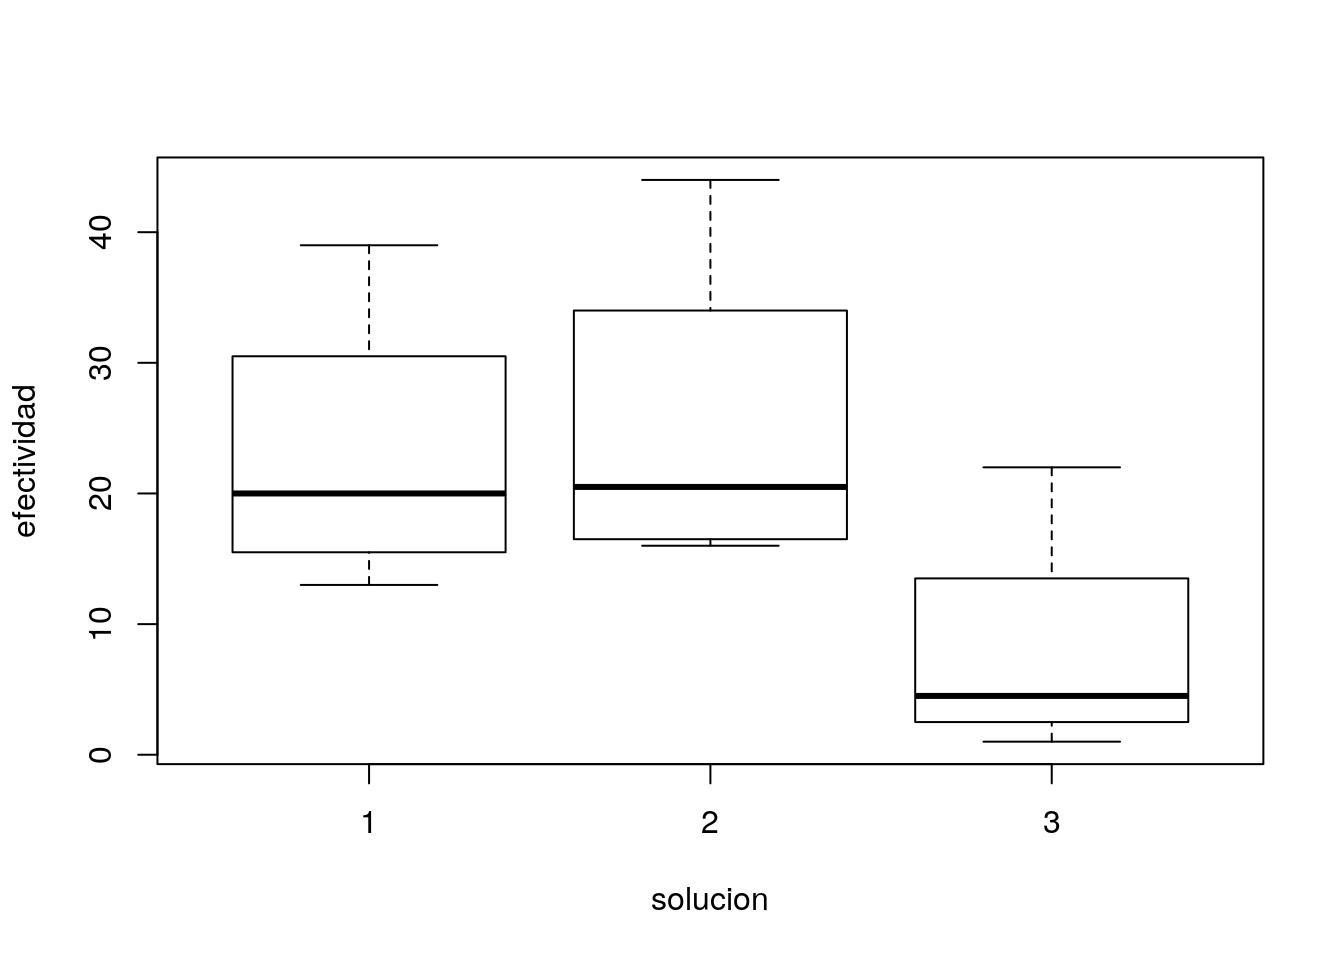
\includegraphics{Introducción_a_los_diseños_experimentales_con_R_files/figure-latex/unnamed-chunk-19-1.pdf}

\begin{Shaded}
\begin{Highlighting}[]
\NormalTok{modelo1<-}\KeywordTok{lm}\NormalTok{(efectividad}\OperatorTok{~}\NormalTok{dias}\OperatorTok{+}\NormalTok{solucion,datos)}
\KeywordTok{anova}\NormalTok{(modelo1)}
\end{Highlighting}
\end{Shaded}

\begin{verbatim}
## Analysis of Variance Table
## 
## Response: efectividad
##           Df Sum Sq Mean Sq F value  Pr(>F)    
## dias       3   1107     369    42.7 0.00019 ***
## solucion   2    704     352    40.7 0.00032 ***
## Residuals  6     52       9                    
## ---
## Signif. codes:  0 '***' 0.001 '**' 0.01 '*' 0.05 '.' 0.1 ' ' 1
\end{verbatim}

\begin{Shaded}
\begin{Highlighting}[]
\NormalTok{citukey <-}\StringTok{ }\KeywordTok{confint}\NormalTok{(}\KeywordTok{glht}\NormalTok{(modelo1, }\DataTypeTok{linfct =} \KeywordTok{mcp}\NormalTok{(}\DataTypeTok{solucion =} \StringTok{"Tukey"}\NormalTok{)))}
\KeywordTok{summary}\NormalTok{(citukey)}
\end{Highlighting}
\end{Shaded}

\begin{verbatim}
## 
##   Simultaneous Tests for General Linear Hypotheses
## 
## Multiple Comparisons of Means: Tukey Contrasts
## 
## 
## Fit: lm(formula = efectividad ~ dias + solucion, data = datos)
## 
## Linear Hypotheses:
##            Estimate Std. Error t value Pr(>|t|)    
## 2 - 1 == 0     2.25       2.08    1.08     0.56    
## 3 - 1 == 0   -15.00       2.08   -7.22   <0.001 ***
## 3 - 2 == 0   -17.25       2.08   -8.30   <0.001 ***
## ---
## Signif. codes:  0 '***' 0.001 '**' 0.01 '*' 0.05 '.' 0.1 ' ' 1
## (Adjusted p values reported -- single-step method)
\end{verbatim}

\begin{Shaded}
\begin{Highlighting}[]
\CommentTok{#En téminos de efectos:}
\NormalTok{op <-}\StringTok{ }\KeywordTok{options}\NormalTok{ (}\DataTypeTok{contrasts=}\KeywordTok{c}\NormalTok{(}\StringTok{"contr.sum"}\NormalTok{,}\StringTok{"contr.poly"}\NormalTok{))}
\NormalTok{modelo2<-}\KeywordTok{lm}\NormalTok{(efectividad}\OperatorTok{~}\NormalTok{dias}\OperatorTok{+}\NormalTok{solucion,datos)}
\KeywordTok{summary}\NormalTok{(modelo2)}
\end{Highlighting}
\end{Shaded}

\begin{verbatim}
## 
## Call:
## lm(formula = efectividad ~ dias + solucion, data = datos)
## 
## Residuals:
##    Min     1Q Median     3Q    Max 
##  -2.58  -1.85  -0.25   1.25   4.42 
## 
## Coefficients:
##             Estimate Std. Error t value Pr(>|t|)    
## (Intercept)   18.750      0.848   22.10  5.6e-07 ***
## dias1         -7.417      1.470   -5.05   0.0023 ** 
## dias2         -2.083      1.470   -1.42   0.2061    
## dias3         -6.750      1.470   -4.59   0.0037 ** 
## solucion1      4.250      1.200    3.54   0.0122 *  
## solucion2      6.500      1.200    5.42   0.0016 ** 
## ---
## Signif. codes:  0 '***' 0.001 '**' 0.01 '*' 0.05 '.' 0.1 ' ' 1
## 
## Residual standard error: 2.9 on 6 degrees of freedom
## Multiple R-squared:  0.972,  Adjusted R-squared:  0.949 
## F-statistic: 41.9 on 5 and 6 DF,  p-value: 0.000137
\end{verbatim}

\begin{Shaded}
\begin{Highlighting}[]
\KeywordTok{par}\NormalTok{(}\DataTypeTok{mfrow=}\KeywordTok{c}\NormalTok{(}\DecValTok{2}\NormalTok{,}\DecValTok{2}\NormalTok{))}
\KeywordTok{plot}\NormalTok{(modelo1)}
\end{Highlighting}
\end{Shaded}

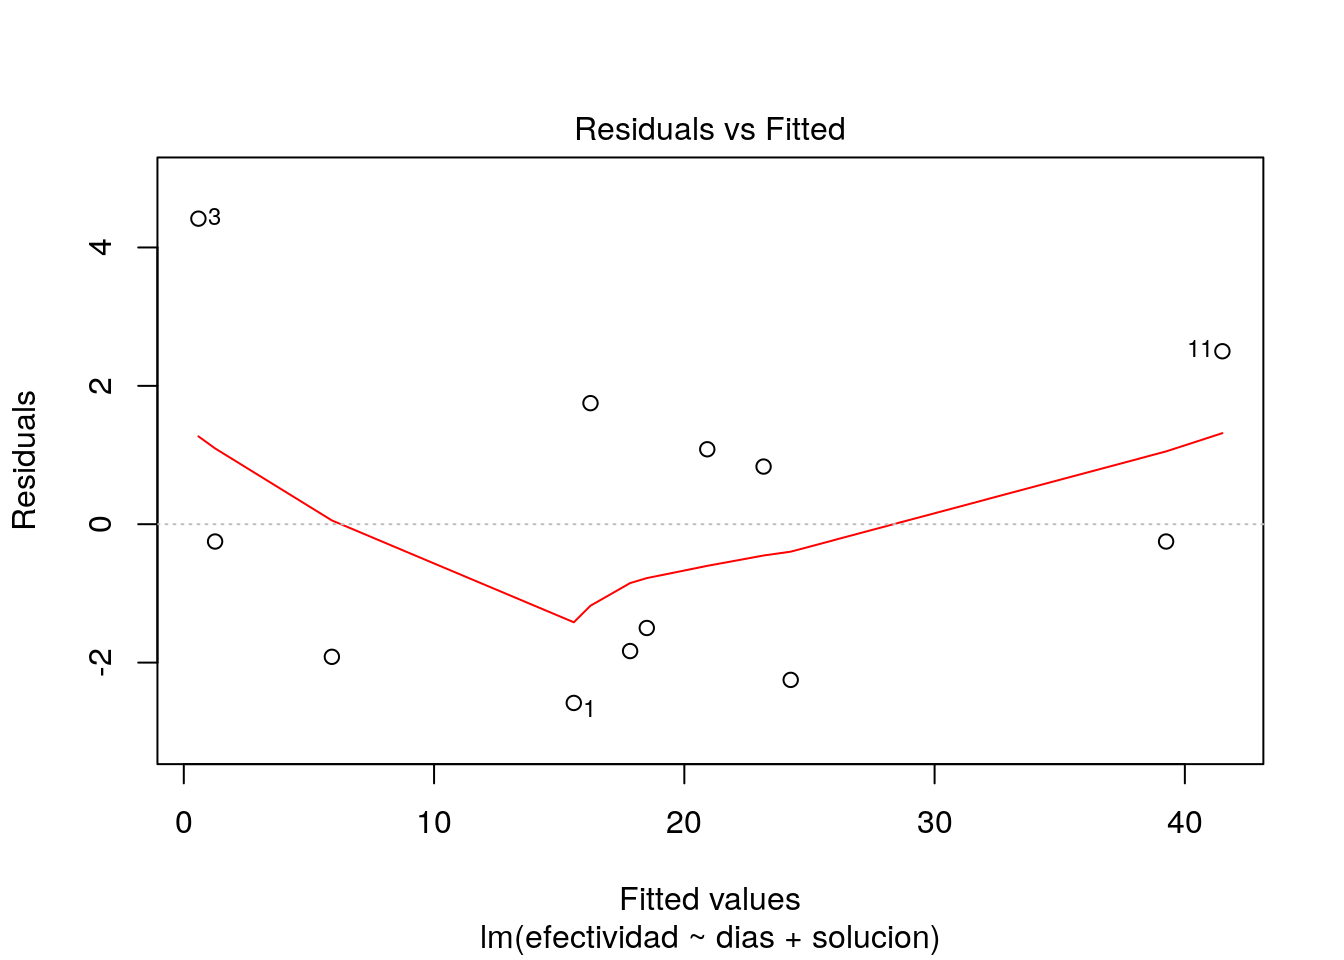
\includegraphics{Introducción_a_los_diseños_experimentales_con_R_files/figure-latex/unnamed-chunk-19-2.pdf}

\section{Actividad}\label{actividad-3}

En un ensayo sobre las ventajas de ejercitarse regularmente, se solicitó
a voluntarios del estudio a participar en la secuencia de ejercicios
aeróbicos de interés, por un determinado tiempo, siendo la secuencia
fijada aleatoriamente para cada participante, Al final de cada prueba se
procedió a medir el gasto de energia por kilómetro recorrido.

\begin{longtable}[]{@{}cccc@{}}
\toprule
Sujeto & Correr & Caminar & Ciclismo\tabularnewline
\midrule
\endhead
1 & 1.4 & 1.1 & 0.7\tabularnewline
2 & 1.5 & 1.2 & 0.8\tabularnewline
3 & 1.8 & 1.3 & 0.7\tabularnewline
4 & 1.7 & 1.3 & 0.8\tabularnewline
5 & 1.6 & 0.7 & 0.1\tabularnewline
6 & 1.5 & 1.2 & 0.7\tabularnewline
7 & 1.7 & 1.1 & 0.4\tabularnewline
8 & 2 & 1.3 & 0.6\tabularnewline
\bottomrule
\end{longtable}

\begin{itemize}
\tightlist
\item
  Plantee un posible esquema de aleatorización.\\
\item
  Analice los datos. Pruebe las hipótesis de interés, use
  \(\alpha=0.05\).
\end{itemize}

\begin{Shaded}
\begin{Highlighting}[]
\CommentTok{# Cargando datos}
\NormalTok{ejercitarse <-}\StringTok{ }\KeywordTok{read.delim}\NormalTok{(}\StringTok{"~/GuiaDisenoExperimR/ejercitarse"}\NormalTok{)}
\KeywordTok{str}\NormalTok{(ejercitarse)}
\end{Highlighting}
\end{Shaded}

\begin{verbatim}
## 'data.frame':    8 obs. of  4 variables:
##  $ Sujeto  : num  1 2 3 4 5 6 7 8
##  $ Correr  : num  1.4 1.5 1.8 1.7 1.6 1.5 1.7 2
##  $ Caminar : num  1.1 1.2 1.3 1.3 0.7 1.2 1.1 1.3
##  $ Ciclismo: num  0.7 0.8 0.7 0.8 0.1 0.7 0.4 0.6
\end{verbatim}

\begin{Shaded}
\begin{Highlighting}[]
\KeywordTok{library}\NormalTok{(reshape)}
\NormalTok{ejercitarse2 <-}\StringTok{ }\KeywordTok{melt}\NormalTok{(ejercitarse, }\DataTypeTok{id=}\StringTok{"Sujeto"}\NormalTok{)}
\KeywordTok{str}\NormalTok{(ejercitarse2)}
\end{Highlighting}
\end{Shaded}

\begin{verbatim}
## 'data.frame':    24 obs. of  3 variables:
##  $ Sujeto  : num  1 2 3 4 5 6 7 8 1 2 ...
##  $ variable: Factor w/ 3 levels "Correr","Caminar",..: 1 1 1 1 1 1 1 1 2 2 ...
##  $ value   : num  1.4 1.5 1.8 1.7 1.6 1.5 1.7 2 1.1 1.2 ...
\end{verbatim}

\chapter{Diseño Cuadrado Latino}\label{diseno-cuadrado-latino}

En esta sección se tiene por objetivos:

\begin{itemize}
\tightlist
\item
  Diseñar un plan para DCL
\item
  Ejecutar el análisis de varianza y evaluación de supuestos
\item
  Realizar pruebas de comparaciones
\end{itemize}

Este diseño es apropiado cuando se presentan dos factores de variación
conocidas en las unidades experimentales que influyen en la respuesta de
interés, siendo posible formar grupos homogéneos (Bloques) de unidades
experimentales de acuerdo a los niveles que toman cada uno de estos
factores de bloqueo. La característica principal de este diseño es que
tan sólo se dispone de una unidad experimental por cada combinación (i,
j) de los niveles de los factores de bloqueo. Es requisito que el número
de grupos homogéneos (bloques) en el primer factor sea igual al número
de bloques en el segundo factor. Esto nos permite representar las
unidades experimentales mediante un cuadrado, donde las filas
representan a un factor de bloqueo (Factor en Filas), las columnas al
otro factor de bloqueo (Factor en Columnas) y cada celda representa una
unidad experimental. El número \(t\) de tratamientos a asignar a las
unidades experimentales es igual al número de filas, así como al de
columnas, siendo el número total de unidades experimentales igual a
\(t^2\) . La asignación aleatoria de los tratamientos a las unidades
experimentales así ordenadas debe cumplir que todos los tratamientos
ocurran en cada fila, e igualmente, en cada columna (modelo balanceado).
Como ejemplo del uso de Cuadrado latino se tiene un experimento que
considera probar cinco distintos fertilizantes en el campo
(Tratamientos), y donde se pueden agrupar las parcelas (unidad
experimental) de acuerdo al grado de pendiente (Factor Filas, cinco
niveles) y al nivel de humedad del suelo (Factor Columnas, cinco
niveles).

\section{Plan de diseño}\label{plan-de-diseno-2}

\begin{Shaded}
\begin{Highlighting}[]
\CommentTok{# Cargando paquetes}
\KeywordTok{library}\NormalTok{(agricolae)}
\NormalTok{trt <-}\StringTok{ }\KeywordTok{c}\NormalTok{(}\StringTok{"A"}\NormalTok{, }\StringTok{"B"}\NormalTok{, }\StringTok{"C"}\NormalTok{, }\StringTok{"D"}\NormalTok{)}
\NormalTok{outdesign <-}\StringTok{ }\KeywordTok{design.lsd}\NormalTok{(trt, }\DataTypeTok{seed=}\DecValTok{543}\NormalTok{, }\DataTypeTok{serie=}\DecValTok{1}\NormalTok{)}
\KeywordTok{print}\NormalTok{(outdesign}\OperatorTok{$}\NormalTok{sketch)}
\end{Highlighting}
\end{Shaded}

\begin{verbatim}
##      [,1] [,2] [,3] [,4]
## [1,] "C"  "A"  "B"  "D" 
## [2,] "D"  "B"  "C"  "A" 
## [3,] "B"  "D"  "A"  "C" 
## [4,] "A"  "C"  "D"  "B"
\end{verbatim}

\begin{Shaded}
\begin{Highlighting}[]
\NormalTok{book3 <-}\StringTok{ }\NormalTok{outdesign}\OperatorTok{$}\NormalTok{book}
\KeywordTok{print}\NormalTok{(book3)}
\end{Highlighting}
\end{Shaded}

\begin{verbatim}
##    plots row col trt
## 1     11   1   1   C
## 2     12   1   2   A
## 3     13   1   3   B
## 4     14   1   4   D
## 5     21   2   1   D
## 6     22   2   2   B
## 7     23   2   3   C
## 8     24   2   4   A
## 9     31   3   1   B
## 10    32   3   2   D
## 11    33   3   3   A
## 12    34   3   4   C
## 13    41   4   1   A
## 14    42   4   2   C
## 15    43   4   3   D
## 16    44   4   4   B
\end{verbatim}

\section{Análisis de Varianza}\label{analisis-de-varianza-2}

El modelo aditivo lineal es:

\[y_{ij}=\mu + \tau_i+\rho_j+\gamma_k+\epsilon_{ij}\]

Cuando los efectos de tratamientos se consideran fijos es de interés
probar:\\
\(H_0:\mu_1=\mu_2=... =\mu_t=\mu\)\\
\(H_1:\)al menos un \(\mu_i \neq \mu\)

\emph{Ejemplo:}

Un ingeniero de tránsito realizó un estudio para comparar el tiempo sin
uso de la luz roja para cinco secuencias distintas de semáforo, el
experimento se llevó a cabo con un diseño cuadrado latino en el que los
dos factores de bloque eran: 1) cinco cruceros elegidos al azar y 2)
cinco períodos. Las cinco secuencias de tratamiento son: a, b, c, d, e.
Se registró el tiempo de la luz roja sin uso (en minutos).(Ejercicio 4.
cap. 8. ``Diseños Experimentales'' (2da edición) R. Kuehl). Los datos se
encuentran en el archivo: ``diseño2.txt''.

\begin{Shaded}
\begin{Highlighting}[]
\NormalTok{datos<-}\KeywordTok{read.table}\NormalTok{(}\StringTok{"diseño2.txt"}\NormalTok{,}\DataTypeTok{header=}\NormalTok{T, }\DataTypeTok{dec=}\StringTok{","}\NormalTok{)}
\KeywordTok{str}\NormalTok{(datos)}
\end{Highlighting}
\end{Shaded}

\begin{verbatim}
## 'data.frame':    25 obs. of  4 variables:
##  $ tiempo   : num  15.2 16.5 12.1 10.7 14.6 33.8 26.5 31.4 34.2 31.7 ...
##  $ crucero  : int  1 2 3 4 5 1 2 3 4 5 ...
##  $ periodo  : int  1 1 1 1 1 2 2 2 2 2 ...
##  $ secuencia: Factor w/ 5 levels "A","B","C","D",..: 1 2 3 4 5 2 3 4 5 1 ...
\end{verbatim}

\begin{Shaded}
\begin{Highlighting}[]
\NormalTok{datos}\OperatorTok{$}\NormalTok{crucero<-}\KeywordTok{as.factor}\NormalTok{(datos}\OperatorTok{$}\NormalTok{crucero)}
\NormalTok{datos}\OperatorTok{$}\NormalTok{periodo<-}\KeywordTok{as.factor}\NormalTok{(datos}\OperatorTok{$}\NormalTok{periodo)}
\KeywordTok{summary}\NormalTok{(datos}\OperatorTok{$}\NormalTok{tiempo)}
\end{Highlighting}
\end{Shaded}

\begin{verbatim}
##    Min. 1st Qu.  Median    Mean 3rd Qu.    Max. 
##      11      17      24      23      29      34
\end{verbatim}

\begin{Shaded}
\begin{Highlighting}[]
\KeywordTok{library}\NormalTok{(mosaic)}
\KeywordTok{favstats}\NormalTok{(tiempo}\OperatorTok{~}\NormalTok{secuencia , }\DataTypeTok{data =}\NormalTok{ datos)}
\end{Highlighting}
\end{Shaded}

\begin{verbatim}
##   secuencia min Q1 median Q3 max mean  sd n missing
## 1         A  15 20     23 32  32   24 7.3 5       0
## 2         B  16 17     27 30  34   25 7.9 5       0
## 3         C  12 14     22 26  26   20 6.9 5       0
## 4         D  11 19     24 27  31   22 8.0 5       0
## 5         E  15 17     26 29  34   24 8.2 5       0
\end{verbatim}

\begin{Shaded}
\begin{Highlighting}[]
\KeywordTok{matrix}\NormalTok{(datos}\OperatorTok{$}\NormalTok{secuencia,}\DecValTok{5}\NormalTok{,}\DecValTok{5}\NormalTok{,}\DataTypeTok{byrow=}\NormalTok{T) }\CommentTok{#visualiza la esctructura correspondiente al cuadrado latino}
\end{Highlighting}
\end{Shaded}

\begin{verbatim}
##      [,1] [,2] [,3] [,4] [,5]
## [1,] "A"  "B"  "C"  "D"  "E" 
## [2,] "B"  "C"  "D"  "E"  "A" 
## [3,] "C"  "D"  "E"  "A"  "B" 
## [4,] "D"  "E"  "A"  "B"  "C" 
## [5,] "E"  "A"  "B"  "C"  "D"
\end{verbatim}

\begin{Shaded}
\begin{Highlighting}[]
\KeywordTok{library}\NormalTok{(ggplot2)}
\KeywordTok{ggplot}\NormalTok{(datos,}\KeywordTok{aes}\NormalTok{(}\DataTypeTok{x=}\NormalTok{crucero,}\DataTypeTok{y=}\NormalTok{tiempo,}\DataTypeTok{shape=}\NormalTok{periodo,}\DataTypeTok{group=}\NormalTok{secuencia))}\OperatorTok{+}\KeywordTok{geom_point}\NormalTok{()}\OperatorTok{+}\KeywordTok{geom_line}\NormalTok{(}\KeywordTok{aes}\NormalTok{(}\DataTypeTok{linetype=}\NormalTok{secuencia))}
\end{Highlighting}
\end{Shaded}

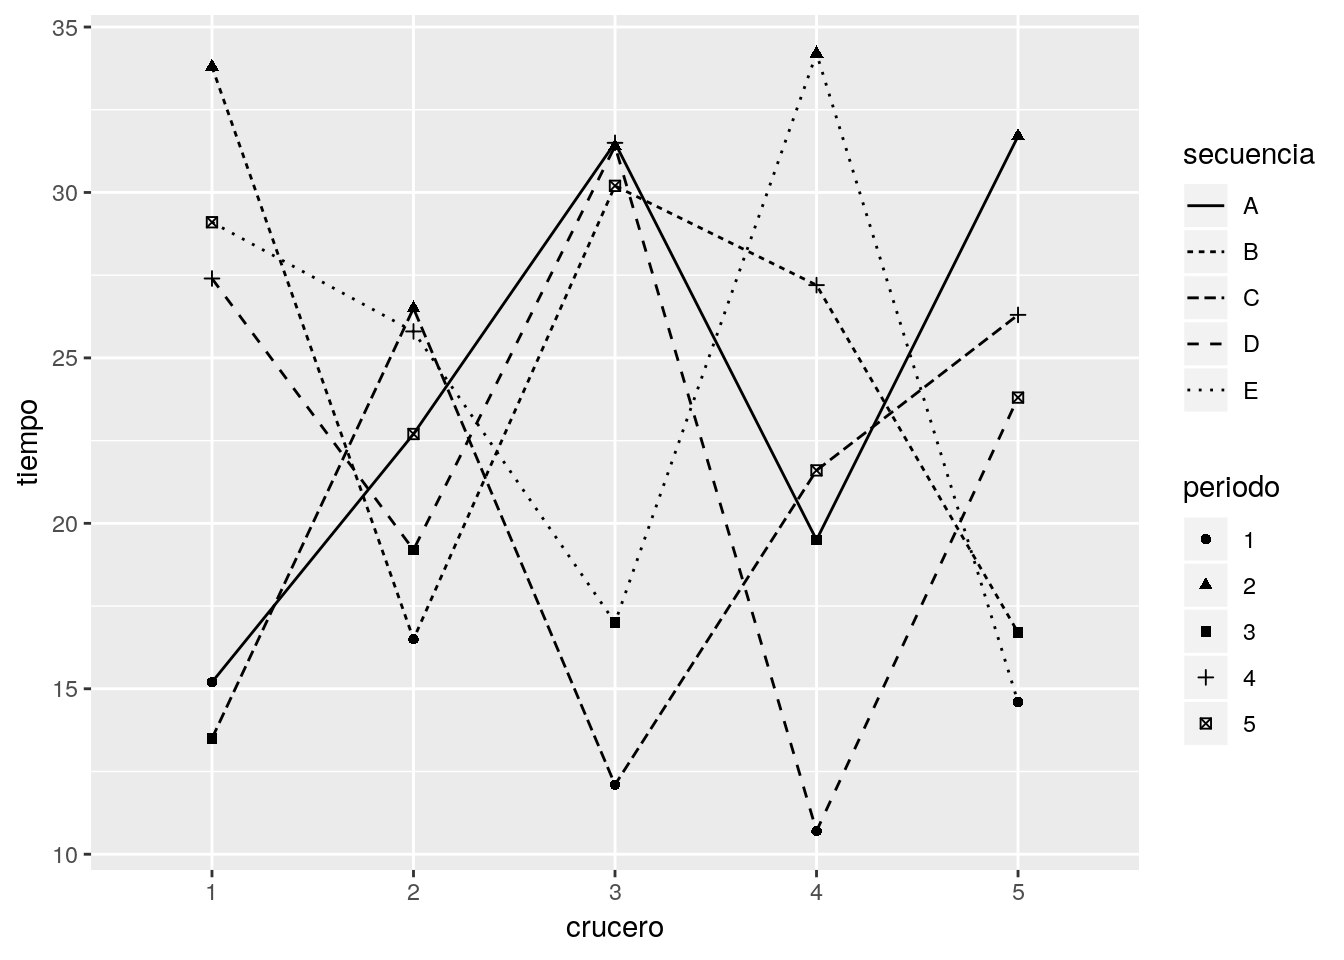
\includegraphics{Introducción_a_los_diseños_experimentales_con_R_files/figure-latex/unnamed-chunk-22-1.pdf}

\begin{Shaded}
\begin{Highlighting}[]
\KeywordTok{ggplot}\NormalTok{(datos,}\KeywordTok{aes}\NormalTok{(}\DataTypeTok{x=}\NormalTok{periodo,}\DataTypeTok{y=}\NormalTok{tiempo,}\DataTypeTok{shape=}\NormalTok{crucero,}\DataTypeTok{group=}\NormalTok{secuencia))}\OperatorTok{+}\KeywordTok{geom_point}\NormalTok{()}\OperatorTok{+}\KeywordTok{geom_line}\NormalTok{(}\KeywordTok{aes}\NormalTok{(}\DataTypeTok{linetype=}\NormalTok{secuencia))}
\end{Highlighting}
\end{Shaded}

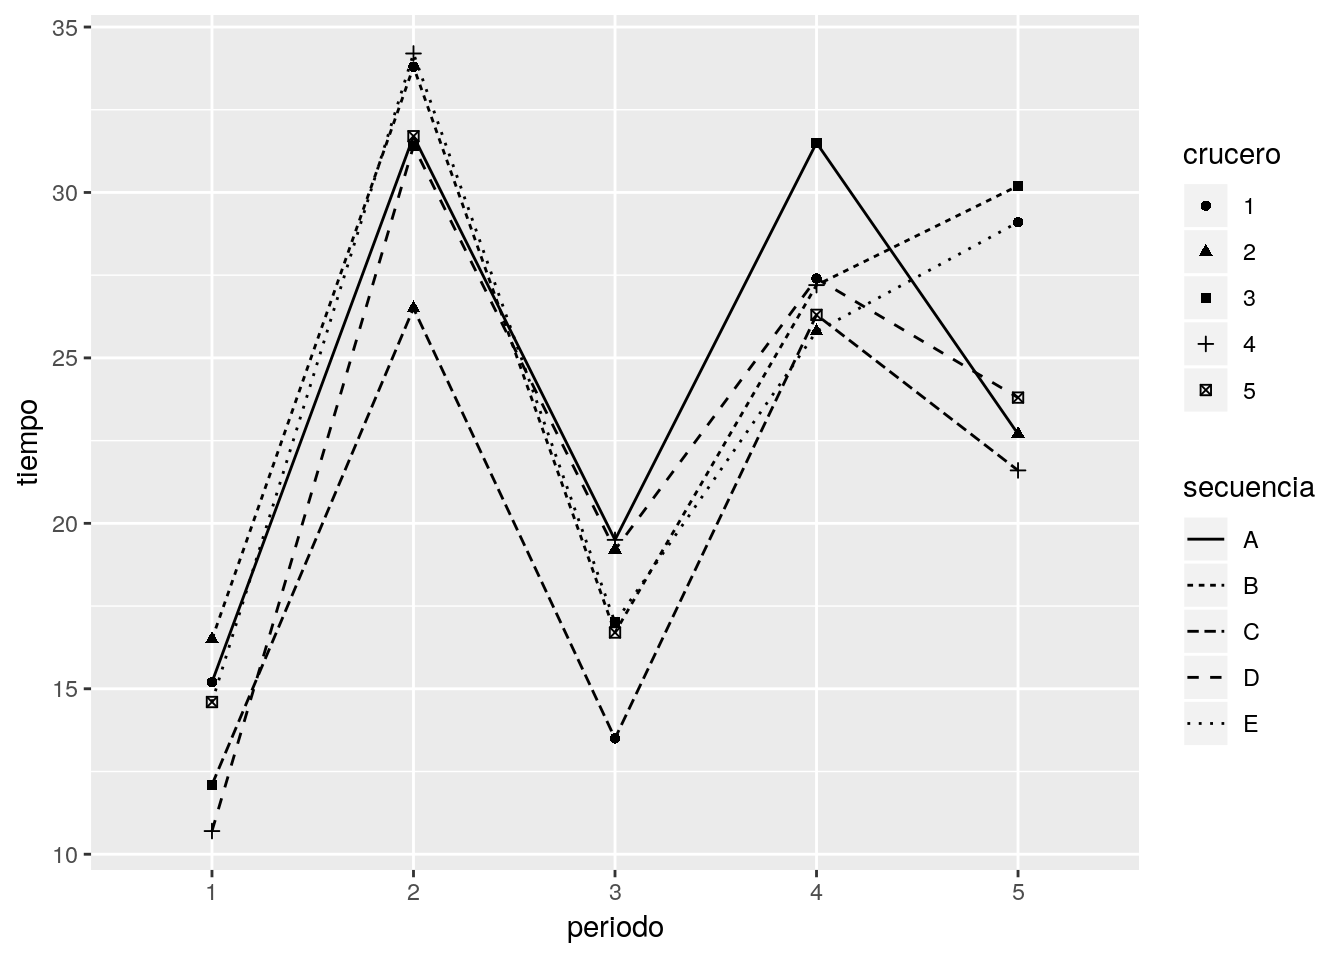
\includegraphics{Introducción_a_los_diseños_experimentales_con_R_files/figure-latex/unnamed-chunk-22-2.pdf}

\begin{Shaded}
\begin{Highlighting}[]
\NormalTok{modelo3<-}\KeywordTok{lm}\NormalTok{(tiempo}\OperatorTok{~}\NormalTok{crucero}\OperatorTok{+}\NormalTok{periodo}\OperatorTok{+}\NormalTok{secuencia,datos)}
\KeywordTok{anova}\NormalTok{(modelo3)}
\end{Highlighting}
\end{Shaded}

\begin{verbatim}
## Analysis of Variance Table
## 
## Response: tiempo
##           Df Sum Sq Mean Sq F value  Pr(>F)    
## crucero    4     18     4.6    0.78    0.56    
## periodo    4   1092   272.9   46.72 3.2e-07 ***
## secuencia  4     76    19.1    3.26    0.05 *  
## Residuals 12     70     5.8                    
## ---
## Signif. codes:  0 '***' 0.001 '**' 0.01 '*' 0.05 '.' 0.1 ' ' 1
\end{verbatim}

\begin{Shaded}
\begin{Highlighting}[]
\KeywordTok{library}\NormalTok{(multcomp)}
\NormalTok{citukey <-}\StringTok{ }\KeywordTok{confint}\NormalTok{(}\KeywordTok{glht}\NormalTok{(modelo3, }\DataTypeTok{linfct =} \KeywordTok{mcp}\NormalTok{(}\DataTypeTok{secuencia =} \StringTok{"Tukey"}\NormalTok{)))}
\KeywordTok{summary}\NormalTok{(citukey)}
\end{Highlighting}
\end{Shaded}

\begin{verbatim}
## 
##   Simultaneous Tests for General Linear Hypotheses
## 
## Multiple Comparisons of Means: Tukey Contrasts
## 
## 
## Fit: lm(formula = tiempo ~ crucero + periodo + secuencia, data = datos)
## 
## Linear Hypotheses:
##            Estimate Std. Error t value Pr(>|t|)  
## B - A == 0     0.76       1.53    0.50     0.99  
## C - A == 0    -4.12       1.53   -2.70     0.11  
## D - A == 0    -1.62       1.53   -1.06     0.82  
## E - A == 0     0.02       1.53    0.01     1.00  
## C - B == 0    -4.88       1.53   -3.19     0.05 *
## D - B == 0    -2.38       1.53   -1.56     0.55  
## E - B == 0    -0.74       1.53   -0.48     0.99  
## D - C == 0     2.50       1.53    1.64     0.50  
## E - C == 0     4.14       1.53    2.71     0.11  
## E - D == 0     1.64       1.53    1.07     0.82  
## ---
## Signif. codes:  0 '***' 0.001 '**' 0.01 '*' 0.05 '.' 0.1 ' ' 1
## (Adjusted p values reported -- single-step method)
\end{verbatim}

\begin{Shaded}
\begin{Highlighting}[]
\NormalTok{op <-}\StringTok{ }\KeywordTok{options}\NormalTok{ (}\DataTypeTok{contrasts=}\KeywordTok{c}\NormalTok{(}\StringTok{"contr.sum"}\NormalTok{,}\StringTok{"contr.poly"}\NormalTok{))}
\NormalTok{modelo3b<-}\KeywordTok{lm}\NormalTok{(tiempo}\OperatorTok{~}\NormalTok{crucero}\OperatorTok{+}\NormalTok{periodo}\OperatorTok{+}\NormalTok{secuencia,datos)}
\KeywordTok{summary}\NormalTok{(modelo3b)}
\end{Highlighting}
\end{Shaded}

\begin{verbatim}
## 
## Call:
## lm(formula = tiempo ~ crucero + periodo + secuencia, data = datos)
## 
## Residuals:
##    Min     1Q Median     3Q    Max 
## -2.784 -1.224 -0.284  1.656  3.636 
## 
## Coefficients:
##             Estimate Std. Error t value Pr(>|t|)    
## (Intercept)   23.128      0.483   47.85  4.5e-15 ***
## crucero1       0.672      0.967    0.70  0.50022    
## crucero2      -0.988      0.967   -1.02  0.32695    
## crucero3       1.312      0.967    1.36  0.19972    
## crucero4      -0.488      0.967   -0.50  0.62285    
## periodo1      -9.308      0.967   -9.63  5.4e-07 ***
## periodo2       8.392      0.967    8.68  1.6e-06 ***
## periodo3      -5.948      0.967   -6.15  4.9e-05 ***
## periodo4       4.512      0.967    4.67  0.00054 ***
## secuencia1     0.992      0.967    1.03  0.32508    
## secuencia2     1.752      0.967    1.81  0.09503 .  
## secuencia3    -3.128      0.967   -3.24  0.00714 ** 
## secuencia4    -0.628      0.967   -0.65  0.52819    
## ---
## Signif. codes:  0 '***' 0.001 '**' 0.01 '*' 0.05 '.' 0.1 ' ' 1
## 
## Residual standard error: 2.4 on 12 degrees of freedom
## Multiple R-squared:  0.944,  Adjusted R-squared:  0.888 
## F-statistic: 16.9 on 12 and 12 DF,  p-value: 1.09e-05
\end{verbatim}

\section{Actividad}\label{actividad-4}

Plantee un diseño cuadrado latino con 5 tratamientos.

En un experimento reportado por Davies (1954), cuatro materiales A, B, C
y D fueron probados en una máquina de desgaste. La respuesta medida es
la pérdida de peso en 0.1mm sobre el período de prueba. La máquina puede
procesar cuatro muestras a la vez y experiencias pasadas indican que
hubieron algunas diferencias debido a la posición ubicada de estas
cuatro muestras. Así también algunas diferencias se sospecha que puede
haberse dado por las diferentes corridas.

\begin{Shaded}
\begin{Highlighting}[]
\KeywordTok{library}\NormalTok{(faraway)}
\NormalTok{datos<-}\KeywordTok{data}\NormalTok{(abrasion,}\DataTypeTok{package=}\StringTok{"faraway"}\NormalTok{)}
\end{Highlighting}
\end{Shaded}

\chapter{Introducción a los Experimentos
factoriales}\label{introduccion-a-los-experimentos-factoriales}

Un experimento factorial es aquel en el que se estudian simultáneamente
varios factores, de modo que los tratamientos se forman por todas las
posibles combinaciones de los niveles de los factores. Un experimento
factorial no constituye un nuevo diseño experimental, sino un diseño
para la formación de los tratamientos. Los experimentos factoriales
pueden ser conducidos bajo los lineamientos de cualquier diseño
experimental tal como el DCA, DBCA o DCL.

\begin{itemize}
\tightlist
\item
  Permite obtener más información que en un experimento de un solo
  factor.
\item
  Todas las unidades intervienen en la estimación de los efectos
  principales y de interacción, por lo que el número de repeticiones
  suele ser elevados.
\item
  Se requiere un mayor número de unidades experimentales que en los
  experimentos simples.
\item
  Todos los niveles de un factor se combinan con todos los niveles de
  los otros factores, sin embargo no siempre todas las combinaciones son
  de interés para el investigador.
\item
  El análisis estadístico y la interpretación de los resultados es más
  complicado que en los experimentos simples con un solo factor.
\end{itemize}

En un experimento factorial un tratamiento corresponde a la combinación
de los niveles de dos o más factores.

\section{Experimentos factorial p x
q}\label{experimentos-factorial-p-x-q}

Un experimento con dos factores con \(p\) y \(q\) niveles en un diseño
Completo al Azar el modelo aditivo lineal es:
\[y_{ijk}=\mu + \alpha_i+\beta_j+\alpha\beta_{ij}+\epsilon_{ijk}\]

Podemos probar las hipótesis de que las medias marginales son todas
iguales, o en términos de los efectos \(\alpha_i\) son todas iguales a
cero, y \(\beta_j\) son todas iguales a cero. Además de probar la
hipótesis de que los efectos de interacción son todos iguales a cero.

¿Cómo hacemos esto, en qué orden y cómo interpretamos estas pruebas?

Uno de los propósitos de un diseño factorial es ser eficiente en la
estimación y prueba de los factores A y B en un solo experimento. A
menudo estamos interesados principalmente en los efectos principales. A
veces, también nos interesa saber si los factores interactúan. En
cualquier caso, la primera prueba que deberíamos hacer es la prueba de
los efectos de interacción.

\emph{Ejemplo:}\\
Se realizó un experimento con un arreglo factorial 2x3 en DBCA en 4
campos de cultivo el efecto en el rendimiento de maíz obtenido con dos
tipos de abono (a1 y a2) y tres dosis (b1=20, b2=30 y b3=40 kg/ha). Los
datos se encuentran en el archivo: ``factorial1.txt''

\begin{Shaded}
\begin{Highlighting}[]
\NormalTok{datos<-}\KeywordTok{read.table}\NormalTok{(}\StringTok{"factorial1.txt"}\NormalTok{,}\DataTypeTok{header=}\NormalTok{T)}
\KeywordTok{str}\NormalTok{(datos)}
\end{Highlighting}
\end{Shaded}

\begin{verbatim}
## 'data.frame':    24 obs. of  4 variables:
##  $ y     : num  1.9 2.3 2 2.1 1.8 2.1 2.4 2.9 2.7 2.4 ...
##  $ B     : int  1 1 1 1 2 2 2 2 3 3 ...
##  $ A     : int  1 1 1 1 1 1 1 1 1 1 ...
##  $ Bloque: int  1 2 3 4 1 2 3 4 1 2 ...
\end{verbatim}

\begin{Shaded}
\begin{Highlighting}[]
\NormalTok{datos}\OperatorTok{$}\NormalTok{Bloque<-}\KeywordTok{as.factor}\NormalTok{(datos}\OperatorTok{$}\NormalTok{Bloque)}
\NormalTok{datos}\OperatorTok{$}\NormalTok{A<-}\KeywordTok{as.factor}\NormalTok{(datos}\OperatorTok{$}\NormalTok{A)}
\NormalTok{datos}\OperatorTok{$}\NormalTok{B<-}\KeywordTok{as.factor}\NormalTok{(datos}\OperatorTok{$}\NormalTok{B)}
\KeywordTok{library}\NormalTok{(mosaic)}
\KeywordTok{favstats}\NormalTok{(y}\OperatorTok{~}\NormalTok{A}\OperatorTok{+}\NormalTok{B , }\DataTypeTok{data =}\NormalTok{ datos)}
\end{Highlighting}
\end{Shaded}

\begin{verbatim}
##   A.B min  Q1 median  Q3 max mean   sd n missing
## 1 1.1 1.9 2.0    2.0 2.2 2.3  2.1 0.17 4       0
## 2 2.1 1.8 1.9    2.1 2.2 2.4  2.1 0.26 4       0
## 3 1.2 1.8 2.0    2.2 2.5 2.9  2.3 0.47 4       0
## 4 2.2 2.7 2.8    3.0 3.3 3.5  3.1 0.35 4       0
## 5 1.3 2.4 2.6    2.8 2.8 2.9  2.7 0.22 4       0
## 6 2.3 2.9 3.0    3.1 3.3 3.4  3.1 0.22 4       0
\end{verbatim}

\begin{Shaded}
\begin{Highlighting}[]
\NormalTok{modelo<-}\KeywordTok{lm}\NormalTok{(y}\OperatorTok{~}\NormalTok{Bloque}\OperatorTok{+}\NormalTok{A}\OperatorTok{+}\NormalTok{B}\OperatorTok{+}\NormalTok{A}\OperatorTok{*}\NormalTok{B,datos)}
\KeywordTok{anova}\NormalTok{(modelo)}
\end{Highlighting}
\end{Shaded}

\begin{verbatim}
## Analysis of Variance Table
## 
## Response: y
##           Df Sum Sq Mean Sq F value  Pr(>F)    
## Bloque     3  0.805   0.268    5.04 0.01298 *  
## A          1  1.000   1.000   18.81 0.00059 ***
## B          2  2.910   1.455   27.35 9.9e-06 ***
## A:B        2  0.563   0.282    5.30 0.01820 *  
## Residuals 15  0.798   0.053                    
## ---
## Signif. codes:  0 '***' 0.001 '**' 0.01 '*' 0.05 '.' 0.1 ' ' 1
\end{verbatim}

\begin{Shaded}
\begin{Highlighting}[]
\KeywordTok{par}\NormalTok{(}\DataTypeTok{mfcol=}\KeywordTok{c}\NormalTok{(}\DecValTok{1}\NormalTok{,}\DecValTok{2}\NormalTok{))}
\KeywordTok{plot}\NormalTok{(modelo, }\DecValTok{1}\OperatorTok{:}\DecValTok{2}\NormalTok{)}
\end{Highlighting}
\end{Shaded}

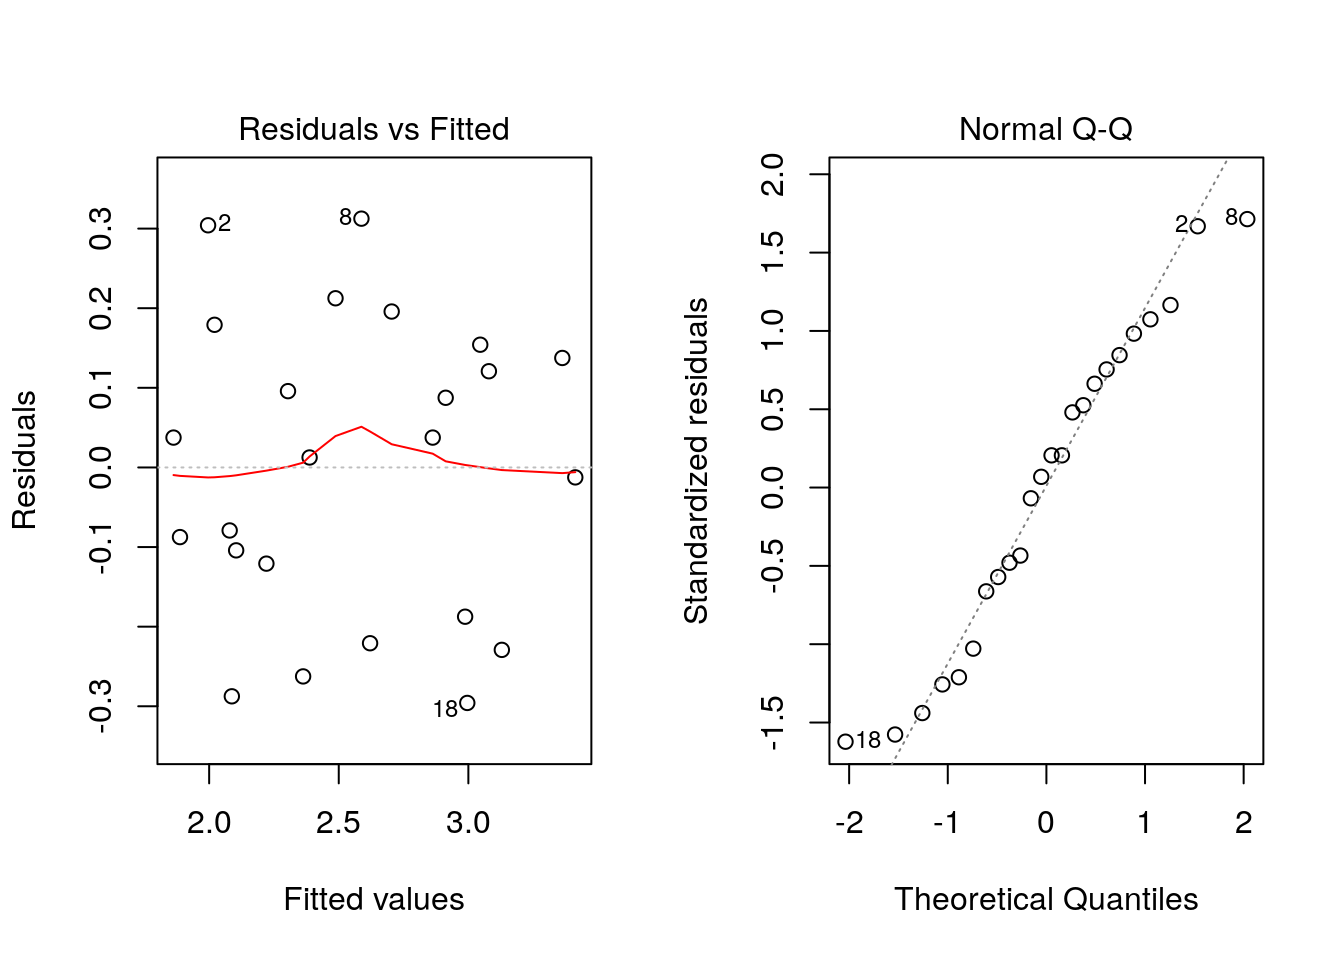
\includegraphics{Introducción_a_los_diseños_experimentales_con_R_files/figure-latex/unnamed-chunk-24-1.pdf}

\begin{Shaded}
\begin{Highlighting}[]
\KeywordTok{library}\NormalTok{(phia)}
\NormalTok{modelo.means <-}\StringTok{ }\KeywordTok{interactionMeans}\NormalTok{(modelo,}\DataTypeTok{factors=}\KeywordTok{c}\NormalTok{(}\StringTok{"A"}\NormalTok{,}\StringTok{"B"}\NormalTok{))}
\NormalTok{modelo.means}
\end{Highlighting}
\end{Shaded}

\begin{verbatim}
##   A B adjusted mean std. error
## 1 1 1           2.1       0.12
## 2 2 1           2.1       0.12
## 3 1 2           2.3       0.12
## 4 2 2           3.1       0.12
## 5 1 3           2.7       0.12
## 6 2 3           3.1       0.12
\end{verbatim}

\begin{Shaded}
\begin{Highlighting}[]
\KeywordTok{plot}\NormalTok{(modelo.means)}
\end{Highlighting}
\end{Shaded}

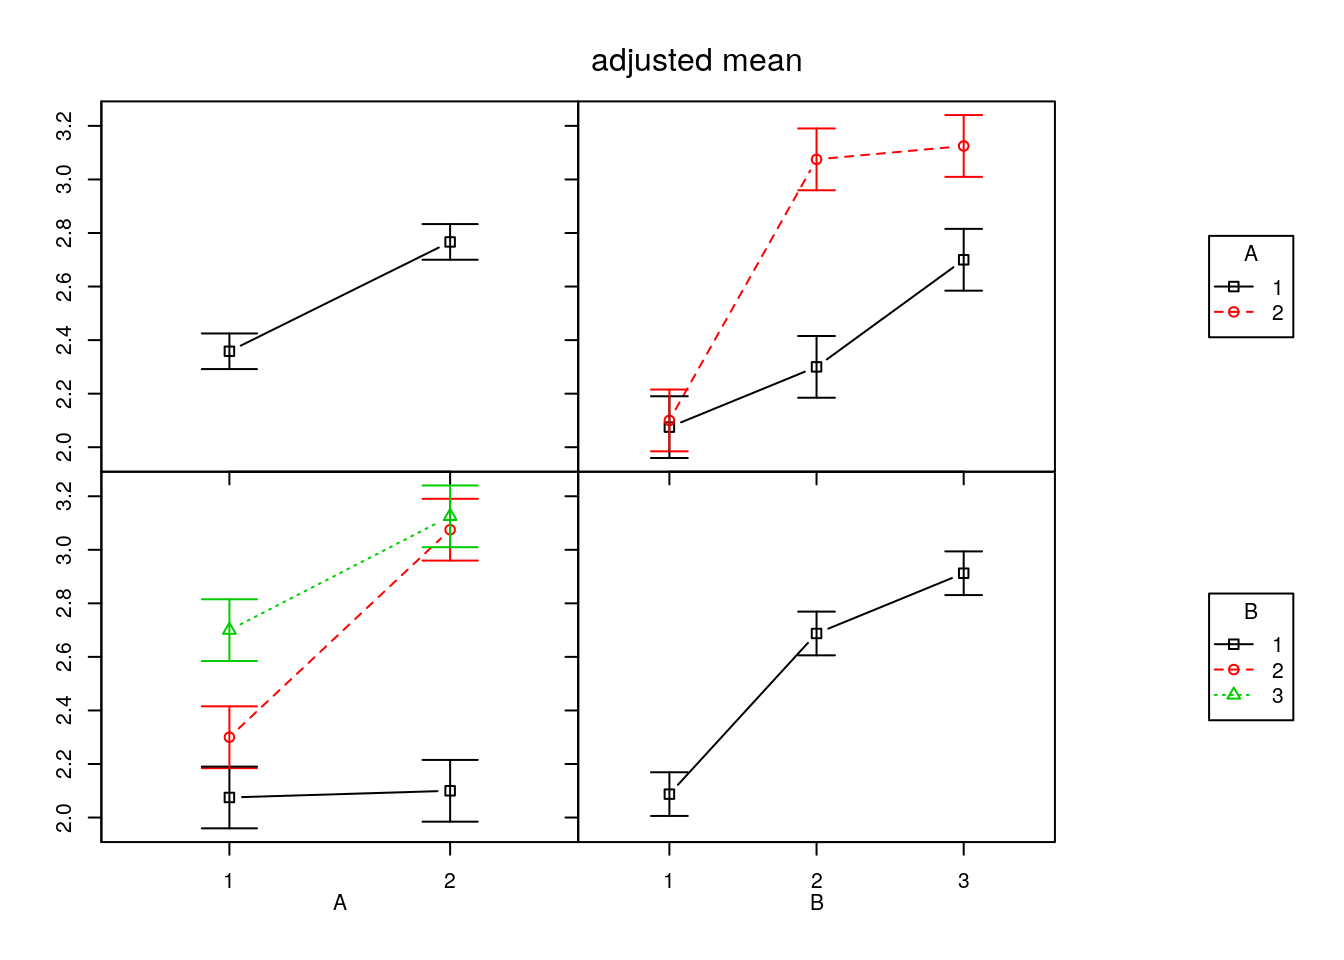
\includegraphics{Introducción_a_los_diseños_experimentales_con_R_files/figure-latex/unnamed-chunk-24-2.pdf}
Es posible observar que al 5\% de significancia hay evidencia de
interacción entre el tipo de abono y dosis. ¿Cómo analizar esta
interacción?

Realizando análisis de Efectos Simples: \emph{Análisis de efectos
simples}

\begin{Shaded}
\begin{Highlighting}[]
\KeywordTok{testInteractions}\NormalTok{(modelo, }\DataTypeTok{fixed=}\StringTok{"A"}\NormalTok{, }\DataTypeTok{across=}\StringTok{"B"}\NormalTok{)}
\end{Highlighting}
\end{Shaded}

\begin{verbatim}
## F Test: 
## P-value adjustment method: holm
##               B1    B2 Df Sum of Sq     F  Pr(>F)    
## 1         -0.625 -0.40  2     0.802  7.54  0.0054 ** 
## 2         -1.025 -0.05  2     2.672 25.11 3.3e-05 ***
## Residuals              15     0.798                  
## ---
## Signif. codes:  0 '***' 0.001 '**' 0.01 '*' 0.05 '.' 0.1 ' ' 1
\end{verbatim}

\begin{Shaded}
\begin{Highlighting}[]
\KeywordTok{testInteractions}\NormalTok{(modelo, }\DataTypeTok{fixed=}\StringTok{"B"}\NormalTok{, }\DataTypeTok{across=}\StringTok{"A"}\NormalTok{)}
\end{Highlighting}
\end{Shaded}

\begin{verbatim}
## F Test: 
## P-value adjustment method: holm
##            Value Df Sum of Sq     F  Pr(>F)    
## 1         -0.025  1     0.001  0.02 0.88021    
## 2         -0.775  1     1.201 22.58 0.00077 ***
## 3         -0.425  1     0.361  6.79 0.03972 *  
## Residuals        15     0.798                  
## ---
## Signif. codes:  0 '***' 0.001 '**' 0.01 '*' 0.05 '.' 0.1 ' ' 1
\end{verbatim}

\emph{Análisis de residuales}

\begin{Shaded}
\begin{Highlighting}[]
\NormalTok{obs.table <-}\StringTok{ }\KeywordTok{xtabs}\NormalTok{(modelo.means}\OperatorTok{$}\StringTok{"adjusted mean"} \OperatorTok{~}\StringTok{ }\NormalTok{A }\OperatorTok{+}\StringTok{ }\NormalTok{B, modelo.means)}
\NormalTok{obs.table<-}\StringTok{ }\KeywordTok{addmargins}\NormalTok{(obs.table,}\DataTypeTok{FUN=}\NormalTok{mean,}\DataTypeTok{quiet=}\OtherTok{TRUE}\NormalTok{)}
\KeywordTok{print}\NormalTok{(obs.table,}\DataTypeTok{digits=}\DecValTok{4}\NormalTok{)}
\end{Highlighting}
\end{Shaded}

\begin{verbatim}
##       B
## A          1     2     3  mean
##   1    2.075 2.300 2.700 2.358
##   2    2.100 3.075 3.125 2.767
##   mean 2.088 2.688 2.913 2.563
\end{verbatim}

\begin{Shaded}
\begin{Highlighting}[]
\NormalTok{res.table <-}\StringTok{ }\NormalTok{obs.table }\OperatorTok{-}\StringTok{ }\NormalTok{obs.table[}\DecValTok{3}\NormalTok{,}\DecValTok{4}\NormalTok{] }\CommentTok{# restando la media}
\NormalTok{res.table <-}\StringTok{ }\KeywordTok{sweep}\NormalTok{(res.table, }\DecValTok{1}\NormalTok{, res.table[,}\DecValTok{4}\NormalTok{]) }\CommentTok{# restando media fila}
\NormalTok{res.table <-}\StringTok{ }\KeywordTok{sweep}\NormalTok{(res.table, }\DecValTok{2}\NormalTok{, res.table[}\DecValTok{3}\NormalTok{,]) }\CommentTok{# restando media comlumna}
\KeywordTok{print}\NormalTok{(res.table, }\DataTypeTok{digits=}\DecValTok{4}\NormalTok{)}
\end{Highlighting}
\end{Shaded}

\begin{verbatim}
##       B
## A              1         2         3      mean
##   1     0.191667 -0.183333 -0.008333  0.000000
##   2    -0.191667  0.183333  0.008333  0.000000
##   mean  0.000000  0.000000  0.000000  0.000000
\end{verbatim}

\begin{Shaded}
\begin{Highlighting}[]
\KeywordTok{testInteractions}\NormalTok{(modelo,}\DataTypeTok{residual=}\KeywordTok{c}\NormalTok{(}\StringTok{"A"}\NormalTok{,}\StringTok{"B"}\NormalTok{))}
\end{Highlighting}
\end{Shaded}

\begin{verbatim}
## F Test: 
## P-value adjustment method: holm
##                           Value Df Sum of Sq    F Pr(>F)  
## 1 (resid.) : 1 (resid.)  0.1917  1     0.441 8.29  0.069 .
## 2 (resid.) : 1 (resid.) -0.1917  1     0.441 8.29  0.069 .
## 1 (resid.) : 2 (resid.) -0.1833  1     0.403 7.58  0.069 .
## 2 (resid.) : 2 (resid.)  0.1833  1     0.403 7.58  0.069 .
## 1 (resid.) : 3 (resid.) -0.0083  1     0.001 0.02  1.000  
## 2 (resid.) : 3 (resid.)  0.0083  1     0.001 0.02  1.000  
## Residuals                       15     0.798              
## ---
## Signif. codes:  0 '***' 0.001 '**' 0.01 '*' 0.05 '.' 0.1 ' ' 1
\end{verbatim}

\begin{Shaded}
\begin{Highlighting}[]
\KeywordTok{matplot}\NormalTok{(}\KeywordTok{t}\NormalTok{(res.table[}\OperatorTok{-}\DecValTok{3}\NormalTok{,}\OperatorTok{-}\DecValTok{4}\NormalTok{]), }\DataTypeTok{type=}\StringTok{"b"}\NormalTok{, }\DataTypeTok{xaxt=}\StringTok{"n"}\NormalTok{, }\DataTypeTok{ylab=}\StringTok{"residuales interacción")}
\StringTok{axis(1, at=1:3, labels=levels(datos$B))}
\end{Highlighting}
\end{Shaded}

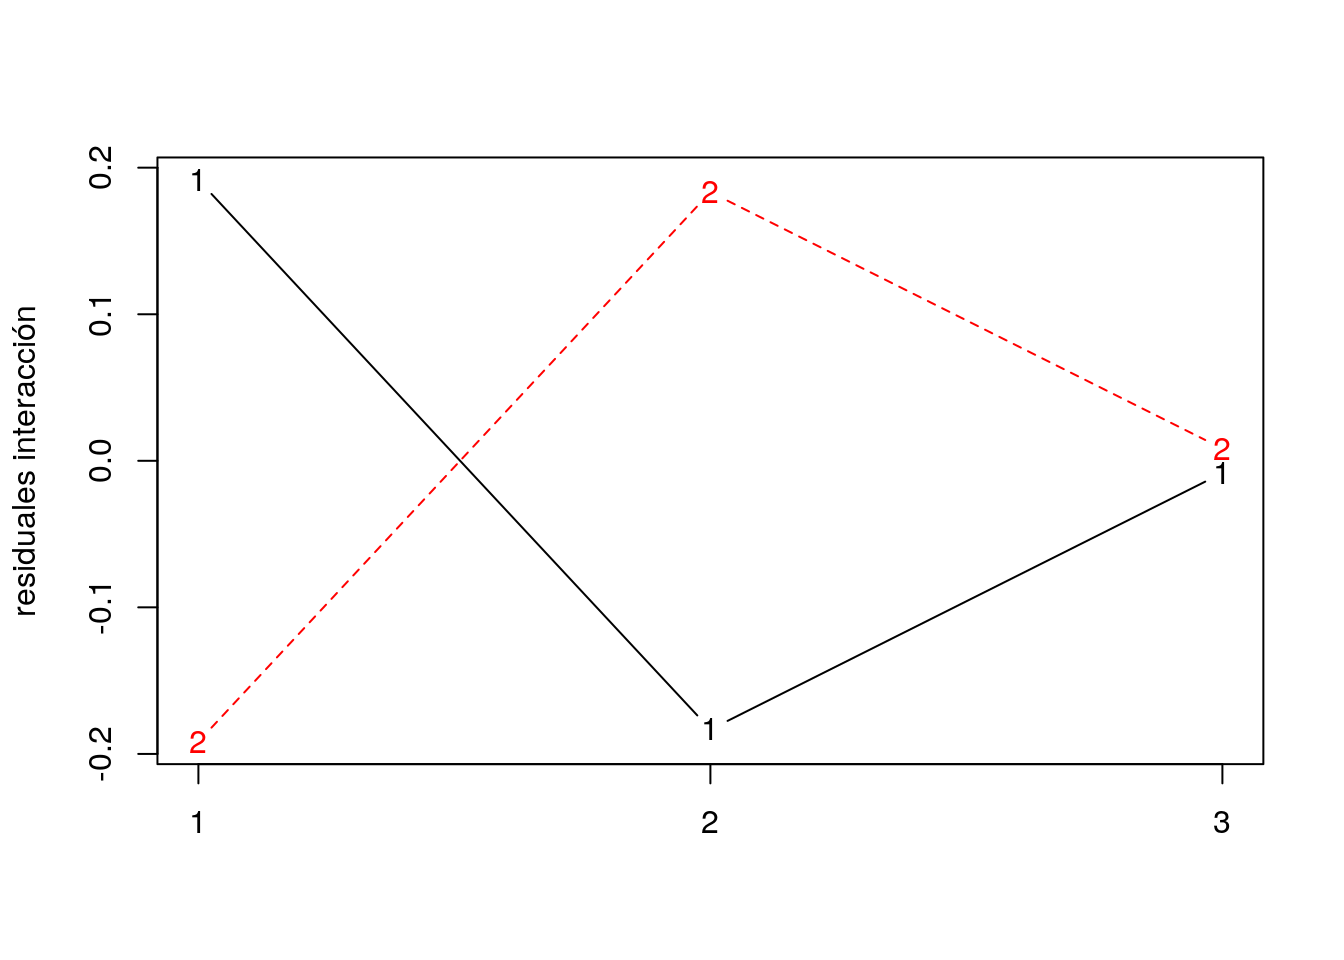
\includegraphics{Introducción_a_los_diseños_experimentales_con_R_files/figure-latex/unnamed-chunk-26-1.pdf}

Utilizando los ejercicios del ejemplo, y con un nivel de significancia
del 1\% hay evidencia de interacción entre el tipo de abono y dosis.
¿Realizaría un análisis de efectos simples o principales?

\emph{Análisis de efectos principales}

\begin{Shaded}
\begin{Highlighting}[]
\NormalTok{model2<-}\KeywordTok{lm}\NormalTok{(y}\OperatorTok{~}\NormalTok{Bloque}\OperatorTok{+}\NormalTok{A}\OperatorTok{+}\NormalTok{B,datos)}
\KeywordTok{library}\NormalTok{(multcomp)}
\NormalTok{citukey <-}\StringTok{ }\KeywordTok{confint}\NormalTok{(}\KeywordTok{glht}\NormalTok{(model2, }\DataTypeTok{linfct =} \KeywordTok{mcp}\NormalTok{(}\DataTypeTok{A =} \StringTok{"Tukey"}\NormalTok{)))}
\KeywordTok{summary}\NormalTok{(citukey)}
\end{Highlighting}
\end{Shaded}

\begin{verbatim}
## 
##   Simultaneous Tests for General Linear Hypotheses
## 
## Multiple Comparisons of Means: Tukey Contrasts
## 
## 
## Fit: lm(formula = y ~ Bloque + A + B, data = datos)
## 
## Linear Hypotheses:
##            Estimate Std. Error t value Pr(>|t|)   
## 2 - 1 == 0    0.408      0.116    3.53   0.0025 **
## ---
## Signif. codes:  0 '***' 0.001 '**' 0.01 '*' 0.05 '.' 0.1 ' ' 1
## (Adjusted p values reported -- single-step method)
\end{verbatim}

\begin{Shaded}
\begin{Highlighting}[]
\NormalTok{citukey <-}\StringTok{ }\KeywordTok{confint}\NormalTok{(}\KeywordTok{glht}\NormalTok{(model2, }\DataTypeTok{linfct =} \KeywordTok{mcp}\NormalTok{(}\DataTypeTok{B =} \StringTok{"Tukey"}\NormalTok{)))}
\KeywordTok{summary}\NormalTok{(citukey)}
\end{Highlighting}
\end{Shaded}

\begin{verbatim}
## 
##   Simultaneous Tests for General Linear Hypotheses
## 
## Multiple Comparisons of Means: Tukey Contrasts
## 
## 
## Fit: lm(formula = y ~ Bloque + A + B, data = datos)
## 
## Linear Hypotheses:
##            Estimate Std. Error t value Pr(>|t|)    
## 2 - 1 == 0    0.600      0.141    4.24   0.0015 ** 
## 3 - 1 == 0    0.825      0.141    5.83   <0.001 ***
## 3 - 2 == 0    0.225      0.141    1.59   0.2766    
## ---
## Signif. codes:  0 '***' 0.001 '**' 0.01 '*' 0.05 '.' 0.1 ' ' 1
## (Adjusted p values reported -- single-step method)
\end{verbatim}

\section{Actividad}\label{actividad-5}

La industria experiemntal examinó el número de roturas de hilo
dependiendo de dos tipos de lana y tres niveles de tensión usando una
máquina de tejer. (Tukey 1977). Los datos se encuentran en la librería
faraway con el nombre de warpbreaks

\begin{Shaded}
\begin{Highlighting}[]
\KeywordTok{library}\NormalTok{(faraway)}
\KeywordTok{str}\NormalTok{(warpbreaks)}
\end{Highlighting}
\end{Shaded}

\begin{verbatim}
## 'data.frame':    54 obs. of  3 variables:
##  $ breaks : num  26 30 54 25 70 52 51 26 67 18 ...
##  $ wool   : Factor w/ 2 levels "A","B": 1 1 1 1 1 1 1 1 1 1 ...
##  $ tension: Factor w/ 3 levels "L","M","H": 1 1 1 1 1 1 1 1 1 2 ...
\end{verbatim}

R.G.D.~Steel, \& Torrie, J.H.(1985). Bioestadística~Principios y
Procedimientos. McGraw Hill, ed Bogotá, Colombia.

Montgomery, D. C. (2005).~Diseño y análisis de experimentos (2nd. Ed).
México: Limusa Wiey.

Kuehl, R. O., (2001). Diseño de experimentos: principios estadísticos
para el diseño y análisis de investigaciones. (2nd Ed). International
Thomson Editores, S.A. de C.V., Mexico, DF.

Ramsey, F. L., \& Schafer, D. W. (2002).~The statistical sleuth: A
course in methods of data analysis. Australia: Duxbury/Thomson Learning

\bibliography{book.bib,packages.bib}


\end{document}
